\documentclass[12pt,oneside,openany,a4paper, %... Layout
afrikaans,english,
%... Global lang drivers
]{memoir}
\usepackage[report, goldenblock]{usthesis}%... Thesis options
\usepackage[afrikaans, english]{babel}
%\SingleSpacing
\usepackage[left=3cm, right=2cm, top=2.5cm, bottom=2.5cm]{geometry}
\usepackage{amsmath}
\usepackage{mathtools}
\numberwithin{equation}{chapter}
\usepackage{bm}
\usepackage{graphicx}
\usepackage{subcaption}
\usepackage{color} % or xcolor
\usepackage{float} %figure location

\renewcommand{\thesection}{\thechapter.\arabic{section}}
\usepackage{tabto}

\usepackage{algorithm}
\usepackage{algpseudocode}
%Watermark
\usepackage{eso-pic}
\newcommand*{\WaterMark}[2][0.15\paperwidth]{%
\AddToShipoutPicture*{\AtTextCenter{%
\parbox[c]{0pt}{\makebox[0pt][c]{%
\includegraphics[width=#1]{#2}}}}}}

%References
\usepackage{usbib}%............................. Bibliography
\bibliographystyle{usmeg-n}%................. Auhor-year style
\addto{\captionsenglish}{\renewcommand{\bibname}{List of References}}

\begin{document}
\pagestyle{plain}
\frontmatter
%TiltePage:
\title{Numerical Integration for Probabilistic Reasoning}
\author{JM.\ Louw}{Jacobus Martin Louw}
\faculty{Faculty of Electrical and Electronic Engineering}
\degree{BEng (E&E)}{Bachelor of Engineering (Electrical and Electronic)}
\ReportDescript{Final Report}
\supervisor{Dr\ CE\ van Daalen}
\frontmatter
%\WaterMark{UScrest-WM}
\TitlePage

\addtocontents{toc}{\protect\setcounter{tocdepth}{-1}}
%Declaration Page
\DeclarationPage

%abstract
\address{Department of Electrical and Electronic Engineering,\\
University of Stellenbosch,\\
Private Bag X1, 7602 Matieland, South Africa.}
\newpage

\tableofcontents
\addtocontents{toc}{\protect\setcounter{tocdepth}{2}}
\pagebreak
\listoffigures

\chapter{List of Acronyms}

\begin{tabbing}
\hspace*{1em}\= \hspace*{5em} \= \hspace*{3em} \= \kill % set the tabbings
\> CPD	\> - \> conditional probability distribution\\
\> EKF	\> - \> extended Kalman filter\\
\> KF	\> - \> Kalman filter\\
\> PDF	\> - \> probability density function\\
\> PGM	\> - \> probabilistic graphical model\\
\> RV \> - \>	random variable\\
\> UKF	\> - \> unscented Kalman filter\\
\end{tabbing}

\chapter{List of Notations}
\begin{tabbing}
\hspace*{1em}\= \hspace*{5em} \= \hspace*{3em} \= \kill % set the tabbings
\> $x$	\> - \> scalar\\
\> $\bm{x}$	\> - \> vector\\
\> $\bm{x}^T$	\> - \> transpose of vector\\
\> $X$ \> - \> matrix\\
\> $X^T$ \> - \> transpose of matrix\\
\> $X^{-1}$ \> - \> inverse of matrix\\
\> $|X|$ \> - \> determinant of matrix\\
\> tr$(X)$ \> - \> trace of matrix\\
\> $p(x)$ \> - \> probability density function\\
\> $\mathcal{N}(\bm{x}; \bm{\mu}, \Sigma)$ \> - \> covariance form\\
\> $\mathcal{C}(\bm{x}; K, \bm{h})$ \> - \> canonical form\\
\> $[0]$ \> - \> zero matrix\\
\> $\bm{0}$ \> - \> zero vector
\end{tabbing}

\chapter{List of Symbols}
\begin{tabbing}
\hspace*{1em}\= \hspace*{5em} \= \hspace*{3em} \= \kill % set the tabbings
\> $C$	\> - \> cluster\\
\> $\bm{h}$	\> - \> potential vector\\
\> $K$	\> - \> information matrix\\
\> $\delta$ \> - \> message in a cluster graph\\
\> $\eta$ \> - \> normalisation coefficient\\
\> $\psi$ \> - \> initial belief cluster\\
\> $\Sigma$ \> - \> covariance matrix
\end{tabbing}
\begin{abstract}
Text in default language ...
\end{abstract}


\mainmatter
\chapter{Introduction}
Robot localisation is the process of estimating where a robot is located relative to its environment. It is essential for autonomous robots to have a precise knowledge of their location in order to navigate their surroundings.

When estimating the location of a robot, a map of the environment and the control input to the robot are usually available. The robot is also generally fitted with sensors which, together with beacons, measure where the robot is located relative to the map. Unfortunately the information of the robot's movements and measurements of its location are uncertain due to noise. The position and orientation of the robot should rather be estimated in a probabilistic manner from the information gathered from the sensors. The localisation techniques must therefore be able to deal with noise and describe the robot's location with a measure of uncertainty.

Probabilistic reasoning of systems with continuous random variables (RV) use integration for various operations. In most nonlinear systems these integrals cannot be calculated analytically and one must use numerical methods. Kalman filters have been used extensively for localisation. Techniques such as the extended Kalman filter use primitive numerical integration that can lead to inaccurate estimations, especially when measurements are also nonlinear. However, there are several alternative numerical techniques available that are more accurate.

A probabilistic graphical model (PGM) is a technique that is used to model systems with uncertainty in an organised manner. It describes the relationship between RVs and allows one to reason about their likelihood based on knowledge that is available to the system. Reasoning about random variables (RVs) in a PGM consists of a number of steps and one can easily identify where integration is used.

The end goal of this project is to investigate different techniques of numerical integration and to implement each technique in a PGM to reason about a nonlinear localisation problem. The techniques of numerical integration will be compared in terms of accuracy and efficiency.
\setcounter{secnumdepth}{2}
\chapter{Gaussian Random Variables}
The Gaussian or normal distribution is commonly used in probability theory, and is amongst other things, very easy to use. Although Gaussian distributions make severe assumptions such as the exponential decay of the distribution away from its mean, they are often surprisingly good estimations for real world distributions. The Gaussian distribution is a very important concept in this report, because all the probability distributions are approximated as Gaussian distributions. Key concepts, features and representations of the Gaussian distribution are discussed in this chapter and is based on the work of Peebles and Shi~\cite{peebles} and Koller and Friedman~\cite{koller}.

\section{Covariance Form}
The value of a random variable (RV) is of a random nature and is drawn from a certain function. The value of a Gaussian RV is drawn from a Gaussian distribution.

The univariate Gaussian distribution is a probability density function (PDF) of a single Gaussian RV. The covariance form fully describes a univariate Gaussian distribution by a mean $\mu$ and variance $\sigma^2$.
The univariate Gaussian distribution of a RV $x$, denoted
\begin{equation}
x\sim\mathcal{N}(\mu,\sigma),
\end{equation}
has a PDF that is defined by
\begin{equation}\label{eq:1}
p(x) = \eta\exp\left[\frac{-(x-\mu)^2}{2\sigma^2}\right],
\end{equation}
with a normalisation coefficient 
\begin{equation}\label{eq:2}
\eta = \frac{1}{\sqrt{2\pi\sigma^2}}.
\end{equation}
The mean parameter $\mu$ describes the location of the peak of the distribution and the variance parameter $\sigma^2$ describes the tempo at which the distribution decays. The probability to draw a value of $X$ out of a Gaussian distribution decreases exponentially as $X$ moves farther away from the mean of the Gaussian distribution. The standard deviation of the Gaussian distribution is denoted as $\sigma$ and it  describes the spread of the PDF.

If $x$ is a continuous RV, then the mean or expectation of $x$ is
\begin{equation}
\mu = \mathcal{E}\left[ x \right] = \int x \cdot p(x)dx.
\end{equation}
The variance of $x$ can be calculated as
\begin{equation}
\begin{split}
\sigma^2 & = \mathcal{E}\left[\left(x - \mathcal{E}[x]\right)^2\right]\\
& = \mathcal{E}[x^2] - (\mathcal{E}[x])^2
\end{split}
\end{equation}
 Figure \ref{fig:gPDF1} indicates the mean $\mu$ and standard deviation $\sigma$ of an univariate Gaussian PDF.
\begin{figure}[H]
  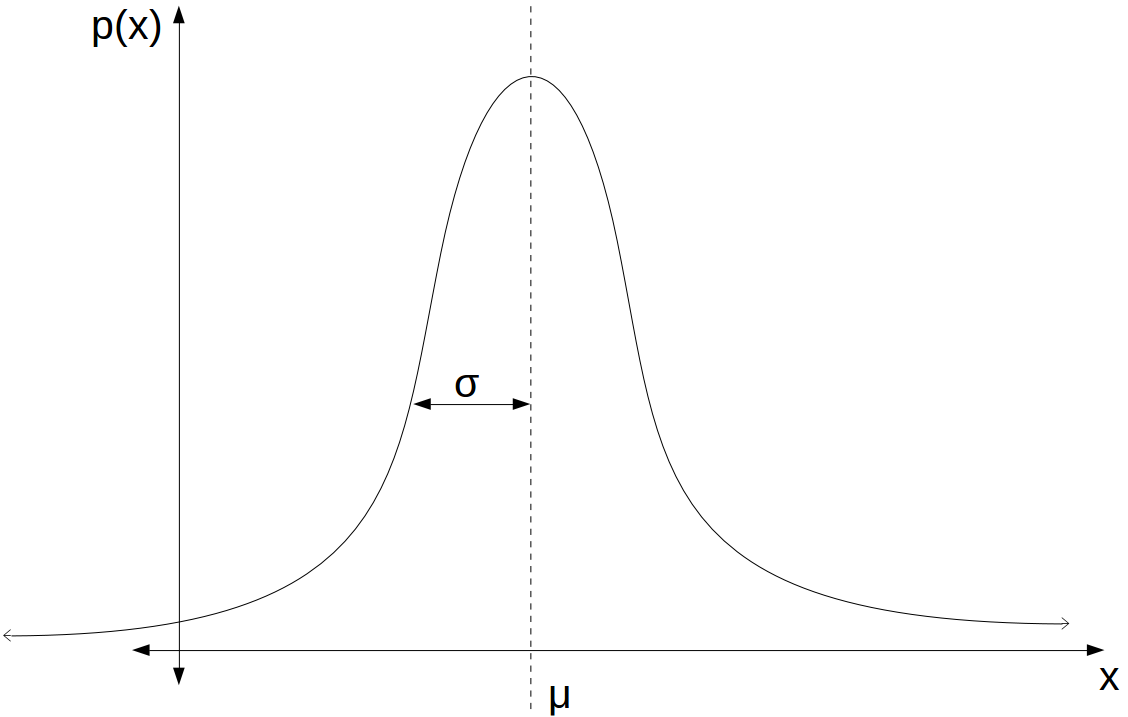
\includegraphics[width=0.6\linewidth]{Figures/univariate.png}
  \centering
  \caption{Univariate Gaussian PDF}
  \label{fig:gPDF1}
\end{figure}
The definition of the Gaussian distribution can be extended to describe the PDF of $N$ random variables (RVs). This is called the multivariate Gaussian distribution. The multivariate Gaussian distribution is described by an $N$-dimensional mean vector $\bm{\mu}$ and an $N\times N$ covariance matrix $\Sigma$. A random vector $\bm{x}$, with $N$ random variables (RVs), is defined as
\begin{equation}
\bm{x} = [x_1\ ...\ x_N]^T,
\end{equation}
where $\bm{x}$ is drawn from a multivariate distribution which is described by a mean vector $\bm{\mu}$ and a covariance matrix $\Sigma$, defined as
\begin{equation}
\bm{x} \sim \mathcal{N}(\bm{x}; \bm{\mu},\Sigma).
\end{equation}
The PDF of $\bm{x}$ is then defined as
\begin{equation}\label{eq:3}
p(\bm{x})  = \eta\exp\left[-\frac{1}{2}(\bm{x}-\bm{\mu})^T\Sigma^{-1}(\bm{x}-\bm{\mu})\right],
\end{equation}
where $\eta$ is a normalisation coefficient and is defined as
\begin{equation}\label{eq:4}
\eta = \frac{1}{(2\pi)^{\frac{N}{2}}|\Sigma|^{\frac{1}{2}}}.
\end{equation}

For this project it is required that $\Sigma$ is positive definite and thus also nonsingular, which guarantees a determinant that is nonzero. Positive definite covariance matrices are also invertible, thus the alternative canonical or information form, which requires $\Sigma^{-1}$, can be used. The canonical form is discussed in the following section.

The mean vector of RV vector $\bm{x}$ is equal to the expectation of $\bm{x}$ and is defined as
\begin{equation}
\bm{\mu} = \mathcal{E}[\bm{x}].
\end{equation}
The covariance matrix $\Sigma$ specifies the correlation between RVs and is equal to
\begin{equation}\label{eq:defCovariance}
\begin{split}
\Sigma & = \mathcal{E}\left[(\bm{x} - \mathcal{E}[\bm{x}])^2\right]\\
& = \mathcal{E}[\bm{xx}^T] - \mathcal{E}[\bm{x}]\mathcal{E}[\bm{x}]^T.
\end{split}
\end{equation}
\subsection{Error Ellipse}The following section is based on an article by Abdi ~\cite{abdi} and on a webpage from "Computer vision for dummies"~\cite{draw_ellipse}.

A multivariate Gaussian distribution with RV vector
\begin{equation}
\bm{x} = [x_1\ x_2]^T
\end{equation}
can be visualised as a series of ellipsoidal contours around the mean vector $\bm{\mu}$. The contours are an indication of the correlation between $x_1$ and $x_2$ and also show the uncertainty of the PDF. Contours close to one another suggest a steep incline and contours that are farther apart suggest a gradual incline in the PDF. Hence, small and concentrated contours represent certain Gaussian distributions and contours that are larger and farther apart represent uncertain Gaussian distributions. The drawing of error ellipses is an effective way to indicate the mean, the uncertainty and the correlation of a 2D Gaussian distribution.

An ellipse has a major axis and a minor axis as shown in Figure \ref{fig:e_ellipse}. The major axis of the error ellipse is always aligned in the direction in which the Gaussian distribution varies most. This direction can be found by determining the eigenvectors of the distribution. Each eigenvector has a corresponding eigenvalue which indicates the spread of the distribution in the direction of the eigenvector. 

We can use eigenvalue decomposition to factorise the covariance matrix $\Sigma$,
\begin{equation}
\Sigma = Q\Lambda Q^{-1}.
\end{equation}
Each column of the eigenvector matrix $Q$ contains an eigenvector $\bm{v}$. $Q$ is defined as
\begin{equation}
Q =
[\bm{v_1} \ \bm{v_2}]
=
\begin{bmatrix}
v_{11} & v_{21}\\
v_{12} & v_{22}
\end{bmatrix}.
\end{equation}
The matrix $\Lambda$ is a diagonal matrix and each of its diagonal entries contains an eigenvalue $\lambda$. $\Lambda$ is defined as 
\begin{equation}
\Lambda =
\begin{bmatrix}
\lambda_1 & 0\\
0 & \lambda_2
\end{bmatrix}.
\end{equation}
An error ellipse of a Gaussian PDF can be specified in terms of confidence levels, which is the probability that a value drawn from the distribution will fall inside the ellipse. Thus, differently sized ellipses can be plotted for different confidence levels. The lengths of the major and minor axes are sequentially specified as $2\sqrt{s\lambda_1}$ and $2\sqrt{s\lambda_2}$, where $\lambda_1 \geq \lambda_2$. The value of $s$ is determined by the confidence level of the error ellipse. In the case of an error ellipse with a confidence level of 95\%, $s$ is set to 5.991. The Chi-Square distribution can be used to find $s$ for other confidence levels, but it is beyond the scope of this document.

The orientation $\alpha$ of the error ellipse is shown in Figure \ref{fig:e_ellipse}. To obtain $\alpha$ we calculate the angle, relative to the x-axis, of the eigenvector with the largest spread. The angle $\alpha$ is defined as
\begin{equation}
\alpha = \arctan\left(\frac{v_{11}}{v_{12}}\right),
\end{equation}
where $\lambda_1 \geq \lambda_2$.

\begin{figure}[H]
  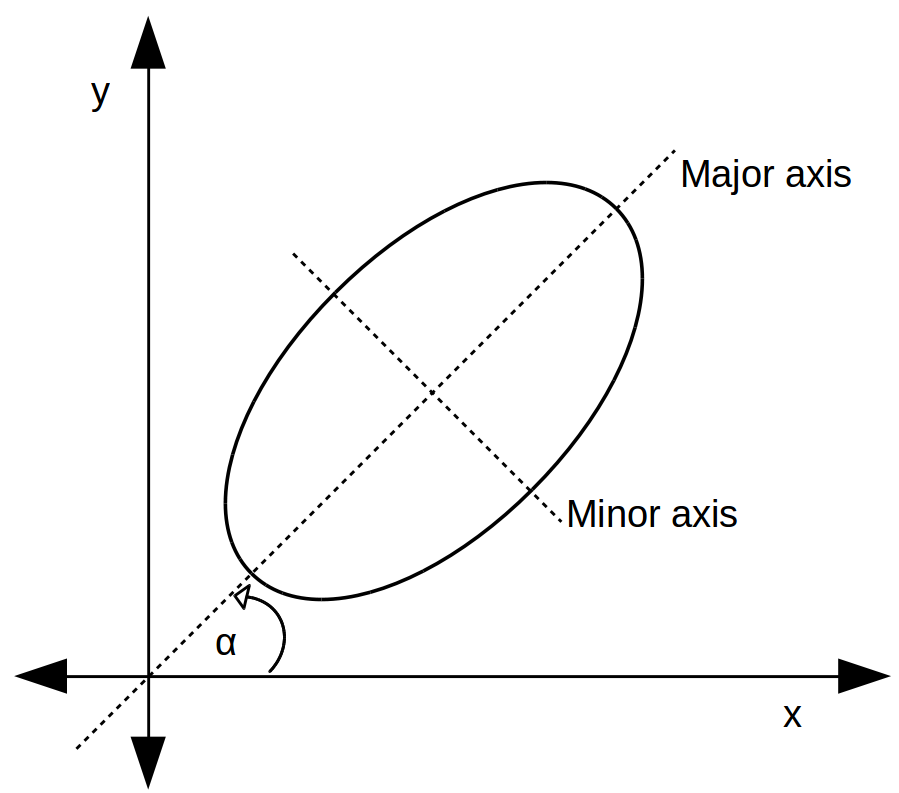
\includegraphics[width=0.5\linewidth]{Figures/e_ellipse.png}
  \centering
  \caption{Error Ellipse}
  \label{fig:e_ellipse}
\end{figure}
\section{Canonical Form}\label{sec:canonical}
The canonical or information form is an alternative way to describe Gaussian distributions. Using the canonical form has benefits, for example that certain operations are easier to perform. It can also be used to represent Gaussian conditional probability densities (CPDs), which will be discussed later in this section. This section is based on the work of Koller and Friedman~\cite{koller} and Schoeman~\citep{JC}.

The definition of the Gaussian distribution, shown in Equation \ref{eq:3}, can be rewritten in the following way
\begin{equation}
\begin{split}\label{eq:pdf_expand}
p(\bm{x}) & = \eta\exp\left[-\frac{1}{2}(\bm{x}-\bm{\mu})^T\Sigma^{-1}(\bm{x}-\bm{\mu})\right]\\
& = \exp\left(-\frac{1}{2}\bm{x}^T\Sigma^{-1}\bm{x} + \bm{\mu}^T\Sigma^{-1}\bm{x} - \frac{1}{2}\bm{\mu}^T\Sigma^{-1}\bm{\mu} + \ln{\eta}\right).
\end{split}
\end{equation}
We define the information matrix as
\begin{equation}\label{eq:defInfoMatrix}
K = \Sigma^{-1},
\end{equation}
the potential vector as
\begin{equation}\label{eq:defPotVec}
\bm{h} = \Sigma^{-1}\bm{\mu},
\end{equation}
and the scalar as
\begin{equation}\label{eq:defScalG}
g = - \frac{1}{2}\bm{\mu}^T\Sigma^{-1}\bm{\mu} + \ln{\eta}.
\end{equation}
We can substitute the definitions from Equation \ref{eq:defInfoMatrix} to Equation \ref{eq:defScalG} into Equation \ref{eq:pdf_expand}, and the define the canonical form as
\begin{equation}\label{eq:defCanonical}
\mathcal{C}(\bm{x}; K,\bm{h},g) = \exp\left(-\frac{1}{2}\bm{x}^TK\bm{x} + \bm{h}^T\bm{x} +g \right).
\end{equation}
Inspecting Equation \ref{eq:defInfoMatrix} to Equation \ref{eq:defScalG} again, it can be seen that one can always determine $g$, if the values of $\bm{h}$ and $K$ is available. This enables us to describe the canonical form in a simpler form, therefore
\begin{equation}
\mathcal{C}(\bm{x}; K,\bm{h},g) \propto \mathcal{C}(\bm{x}; K,\bm{h}).
\end{equation}
One can easily recover the covariance parameters from the canonical parameters, where
\begin{equation}
\Sigma = K^{-1}
\end{equation}
and
\begin{equation}
\bm{\mu} = \Sigma\bm{h}.
\end{equation}
If $K$ is not invertible and the covariance can not be recovered, the canonical form is therefore more general than the covariance form.

It can be seen from the above that it is very easy to convert between the canonical and covariance forms. 
\subsection{Operations using the Canonical Form}
This section will cover useful operations using the canonical forms. 

Extending and rearranging the scopes of canonical forms may be necessary before doing operations, because it is important that the scopes of canonical forms are identical when doing operations. 
\subsubsection{Extending the Scope of a Canonical Form:}
The scope of a canonical form can be extended by adding zero entries to the matrix $K$ and vector $\bm{h}$. The scope of a canonical form of a $M$ sized random vector $\bm{x}$, can easily be extended to the size of $M + N$, by adding zeros in the following way:
\begin{equation}
\mathcal{C}\left(\bm{x};K,\bm{h}\right)
=
\mathcal{C}\left(
\begin{bmatrix}
\bm{x}\\
\bm{y}
\end{bmatrix};
\begin{bmatrix}
K & [0]_{M \times N}\\
[0]_{N \times M} & [0]_{N \times N}\\
\end{bmatrix},
\begin{bmatrix}
\bm{h}\\
\bm{0}
\end{bmatrix}
\right).
\end{equation}
\subsubsection{Rearranging the Scope of a Canonical Form:}
The scope of a canonical form can be rearranged by changing the order of the rows and columns of the matrix $K$ and repositioning the entries of the vector $\bm{h}$:
\begin{equation}
\mathcal{C}\left(
\begin{bmatrix}
\bm{x}\\
\bm{y}\\
\bm{z}
\end{bmatrix};
\begin{bmatrix}
K_{\bm{xx}} & K_{\bm{xy}} & K_{\bm{xz}}\\
K_{\bm{yx}} & K_{\bm{yy}} & K_{\bm{yz}}\\
K_{\bm{zx}} & K_{\bm{zy}} & K_{\bm{zz}}
\end{bmatrix},
\begin{bmatrix}
\bm{h_x}\\
\bm{h_y}\\
\bm{h_z}
\end{bmatrix}
\right)
=
\mathcal{C}\left(
\begin{bmatrix}
\bm{y}\\
\bm{x}\\
\bm{z}
\end{bmatrix};
\begin{bmatrix}
K_{\bm{yy}} & K_{\bm{yx}} & K_{\bm{yz}}\\
K_{\bm{xy}} & K_{\bm{xx}} & K_{\bm{xz}}\\
K_{\bm{zy}} & K_{\bm{zx}} & K_{\bm{zz}}
\end{bmatrix},
\begin{bmatrix}
\bm{h_y}\\
\bm{h_x}\\
\bm{h_z}
\end{bmatrix}
\right).
\end{equation}
\subsubsection{Multiplication of Canonical Forms:}
If the scopes of two canonical forms are identical, one can multiply them by simply adding the $K$ and $\bm{h}$ parameters of the two canonical forms:
\begin{equation}\label{eq:10}
\mathcal{C} (\bm{x}; K_{\bm{x}},\bm{h_x}) \times \mathcal{C} (\bm{y}; K_{\bm{y}},\bm{h_y})= \mathcal{C} (\bm{z};K_{\bm{x}} + K_{\bm{y}}, \bm{h_x} + \bm{h_y}).
\end{equation}
%\subsubsection{Division of canonical forms:}
%Again, it important that the scopes of the distributions are identical.
%\begin{equation}\label{eq:11}
%\frac{\mathcal{C}(K_1,\bm{h_1},g_1)}{\mathcal{C}(K_2,\bm{h_2},g_2)} = %\mathcal{C}(K_1 - K_2,\bm{h_1} - \bm{h_2},g_1 - g_2)
%\end{equation}
\subsubsection{Marginalisation of a Canonical Form:}
A marginal distribution can be found by integrating over a subset of variables, for example the marginal distribution over $\bm{x}$ can be found by integrating over $\bm{y}$. Let $\mathcal{C}(\bm{x},\bm{y};K,\bm{h})$ be a canonical form with subsets $\bm{x}$ and $\bm{y}$ where
\begin{equation}
K = 
\begin{bmatrix}
K_{\bm{xx}} & K_{\bm{xy}}\\
K_{\bm{yx}} & K_{\bm{yy}}
\end{bmatrix}
\end{equation}
and
\begin{equation}
\ h = 
\begin{bmatrix}
h_{\bm{x}} \\
h_{\bm{y}}
\end{bmatrix}.
\end{equation}
To obtain the marginal distribution over $\bm{x}$, we have to find the integral over $\bm{y}$. Therefore the marginal distribution over $\bm{x}$ is
\begin{equation}
\int\mathcal{C}(\bm{x},\bm{y};K,\bm{h})d\bm{y} = \mathcal{C}(\bm{x};K',\bm{h}'),
\end{equation}
 where
\begin{equation}
K' = K_{\bm{xx}} - K_{\bm{xy}}K_{\bm{yy}}^{-1}K_{\bm{yx}}
\end{equation}
and
\begin{equation}
\bm{h'} = \bm{h}_{\bm{x}} - K_{\bm{xx}}K_{\bm{yy}}^{-1}\bm{h}_{\bm{y}}.
\end{equation}
It is important that $K_{\bm{yy}}$ is positive definite for the result to be finite.
\subsubsection{Reduction with Evidence:}
Let $\mathcal{C}(\bm{x},\bm{y};K,\bm{h})$ be a canonical form with subsets $\bm{x}$ and $\bm{y}$. If the value of subset $\bm{y}$ is known to be $\bm{Y}$, then the canonical form can be reduced to $\mathcal{C}(\bm{x}; K',\bm{h}')$, where
\begin{equation}
K' = K_{\bm{xx}},
\end{equation}
\begin{equation}
\bm{h'} = \bm{h}_{\bm{x}} - K_{\bm{xy}}\bm{Y},
\end{equation}

The operations discussed above are very simple to perform and will be used in the following chapters.
\subsection{Conditional Probability Distributions in the Canonical Form}
One of the advantages of the canonical form is that it is possible to represent conditional probability distributions (CPDs).

The CPD $p(\bm{y}|\bm{x})$ is a distribution of the vector $\bm{y}$, given we know the value of the vector $\bm{x}$, and is defined as
\begin{equation}
p(\bm{y}|\bm{x}) = \frac{p(\bm{y},\bm{x})}{p(\bm{x})}.
\end{equation}

If the arguments of the CPD $p(\bm{y}|\bm{x})$ can be described by a linear function, therefore
\begin{equation}
\bm{y} = F\bm{x} + \bm{g} + \bm{n},
\end{equation}
where the noise $\bm{n}$ is described as
\begin{equation}
\bm{n} \sim \mathcal{N}(\bm{n}; \bm{0}, \Sigma_n),
\end{equation}
then the PDF of $p(\bm{y}|\bm{x})$ is defined as 
\begin{equation}
\label{eq:30}
\begin{split}
p(\bm{y}|\bm{x}) & = \mathcal{N}(\bm{y}; F\bm{x} + \bm{g}, \Sigma) \\
& = \eta\exp\left[-\frac{1}{2}(\bm{y} - (F\bm{x} + \bm{g}))^T\Sigma^{-1}(\bm{y}-(F\bm{x} + \bm{g}))\right].
\end{split}
\end{equation}
A part of Equation \ref{eq:30} can be rewritten as 
\begin{equation}\label{eq: rewrite}
\begin{split}
\bm{y} - (F\bm{x} + \bm{g}) & =
\begin{bmatrix}
I&-F&-I
\end{bmatrix}
\begin{bmatrix}
\bm{y}\\
\bm{x}\\
\bm{g}
\end{bmatrix}\\
& =
\begin{bmatrix}
I\\-F^T\\-I
\end{bmatrix}^T
\begin{bmatrix}
\bm{y}\\
\bm{x}\\
\bm{g}
\end{bmatrix}.
\end{split}
\end{equation}
Substituting Equation \ref{eq: rewrite} into Equation \ref{eq:30} gives
\begin{equation}
\label{eq:32}
\begin{split}
p(\bm{y}|\bm{x}) = \eta\exp\left[-\frac{1}{2}
\begin{bmatrix}
\bm{y}\\
\bm{x}\\
\bm{g}
\end{bmatrix}^T
\begin{bmatrix}
I\\-F^T\\-I
\end{bmatrix}
\Sigma^{-1}
\begin{bmatrix}
I\\-F^T\\-I
\end{bmatrix}^T
\begin{bmatrix}
\bm{y}\\
\bm{x}\\
\bm{g}
\end{bmatrix}
\right].
\end{split}
\end{equation}
We now define a new combined random vector
\begin{equation}\label{eq:ranVec}
\bm{w} = 
\begin{bmatrix}
\bm{y}\\
\bm{x}\\
\bm{g}

\end{bmatrix}
\end{equation}
and an information matrix
\begin{equation}\label{eq:newK}
K' =
\begin{bmatrix}
I\\-F^T\\-I
\end{bmatrix}
\Sigma^{-1}
\begin{bmatrix}
I\\-F^T\\-I
\end{bmatrix}^T.
\end{equation}
We can substitute Equation \ref{eq:ranVec} and Equation \ref{eq:newK} into Equation \ref{eq:32} which gives
\begin{equation}
\label{eq:35}
\begin{split}
p(\bm{y}|\bm{x}) = \eta\exp\left[-\frac{1}{2}
\bm{w}^T
K'
\bm{w}
\right].
\end{split}
\end{equation}
We can now use Equation \ref{eq:defCanonical} to write the conditional distribution of Equation \ref{eq:35} in the canonical form as follows
\begin{equation}\label{eq:linCan}
p(\bm{y}|\bm{x}) \propto \mathcal{C}(\bm{w}; K', \bm{0})\\
 =\mathcal{C}\left(
\begin{bmatrix}
\bm{y} \\
\bm{x} \\
\bm{g}
\end{bmatrix};
\begin{bmatrix}
I\\
-F^T\\
-I
\end{bmatrix}
\Sigma^{-1}
\begin{bmatrix}
I\\
-F^T\\
-I
\end{bmatrix}^T
, \bm{0}
\right)
\end{equation}
The parameter $\bm{g}$ is a constant and can be used as evidence to reduce the canonical form in Equation \ref{eq:linCan}, therefore
\begin{equation}\label{eq:conCanResult}
\begin{split}
\mathcal{C}(\bm{w}; K', \bm{0})& =\mathcal{C}\left(
\begin{bmatrix}
\bm{y} \\
\bm{x} \\
\end{bmatrix};
\begin{bmatrix}
I\\
-F^T
\end{bmatrix}
\Sigma^{-1}
\begin{bmatrix}
I\\
-F^T
\end{bmatrix}^T,
\begin{bmatrix}
I\\
-F^T
\end{bmatrix}
\Sigma^{-1}\bm{g}
\right)\\
& =\mathcal{C}\left(
\begin{bmatrix}
\bm{y} \\
\bm{x} \\
\end{bmatrix};
\begin{bmatrix}
\Sigma^{-1}  &  -\Sigma^{-1}F\\
-F^T\Sigma^{-1} & F^T\Sigma^{-1}F
\end{bmatrix}
, 
\begin{bmatrix}
-\Sigma^{-1}\bm{g}\\
-F^T\Sigma^{-1}\bm{g}
\end{bmatrix}
\right).
\end{split}
\end{equation}
The canonical form can therefore also be used to represent linear Gaussian conditional probability distributions (CPDs). The canonical form is used in later chapters to do operations on various Gaussian distributions.

\chapter{Motion Models}\label{chap:motionModel}
Before locating a robot, it is important to model the way the robot moves. A simple linear motion model will be described, which will later be used to illustrate basic principles when estimating the location of a linear moving robot. In practice the movement of a robot is seldom linear, therefore a more complex nonlinear motion model will also have to be explored. This chapter is based on the work of Thrun, Burgard and Fox~\citep{thrun}.
\section{Basic Concepts}
The motion model describes $p(\bm{x}_t|\bm{u}_t,\bm{x}_{t-1})$, which is the state transition probability density function (PDF). This is important and is used in the \textit{prediction step} of the Bayes filter, discussed in Chapter \ref{chap:kalmanFilter}. The material will cover kinematics in a stochastic form. Robot motion will be limited to planar movement to make it easier to convey concepts or ideas to the reader. Note that the theory discussed is not limited to planar movement and can easily be extended to three dimensions.

The kinematic state of a robot moving in a plane can be described by three variables which is referred to as the pose of the robot.
The pose is defined as
\begin{equation}
\bm{x_t} =
\begin{bmatrix}
x_t\\
y_t\\
\theta_t
\end{bmatrix}.
\end{equation}
As shown in Figure \ref{fig:pose_robot}, $x_t$ is the x-coordinate, $y_t$ is the y-coordinate and $\theta_t$ is the orientation of the robot at time $t$.

\begin{figure}[H]
  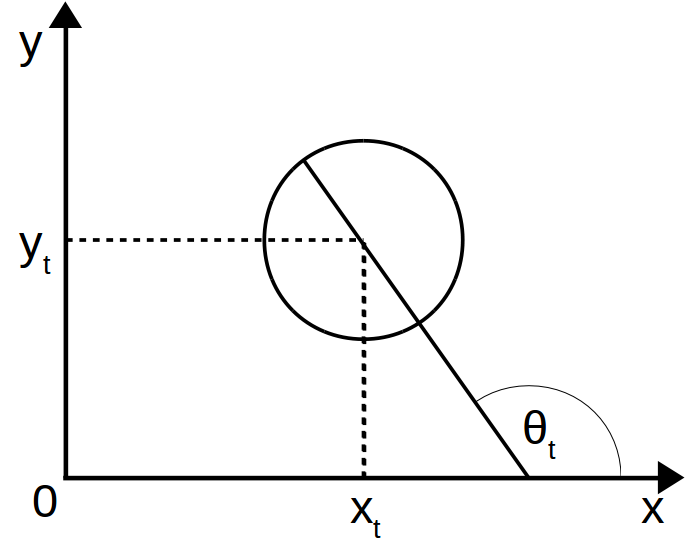
\includegraphics[width=0.4\linewidth]{Figures/pose_robot.png}
  \centering
  \caption{Robot pose}
  \label{fig:pose_robot}
\end{figure}
\section{Linear Motion Model}\label{sec:linearMotionModel}
This section describes the linear motion model. The parameter $\theta_t$ is omitted from the pose  and therefore the kinematic state of the robot is described only by a location
\begin{equation}
\bm{y_t} =
\begin{bmatrix}
x_t\\
y_t
\end{bmatrix}.
\end{equation}

The motion of the robot is independent of its orientation and can be controlled with two translational velocities in a control vector  $\bm{u}_t$, defined as
\begin{equation}
\bm{u_t} = 
\begin{bmatrix}
v_{x,t}\\
v_{y,t}
\end{bmatrix},
\end{equation}
where $v_{x,t}$ is the velocity in the x-direction and $v_{y,t}$ is the velocity in the y-direction at time $t$.

The position $\bm{y_t}$ of the robot at time $t$ can be described by a linear function in the form of
\begin{equation}\label{eq:lineartrans}
\bm{y_t} = A_t \bm{y_{t - 1}} + B_t \bm{u_t} + \bm{\varepsilon}_t,
\end{equation}
where
\begin{equation}
A_t =
\begin{bmatrix}
1 & 0\\
0 & 1
\end{bmatrix},
\end{equation}
\begin{equation}
B_t = \begin{bmatrix}
\Delta t & 0\\
0 & \Delta t
\end{bmatrix},
\end{equation}
and the noise is described as a Gaussian distribution
\begin{equation}
\bm{\varepsilon}_t \sim \mathcal{N}(\bm{\varepsilon}_t; 0, R_t).
\end{equation}
The covariance matrix $R_t$ is defined as
\begin{equation}
R_t = 
\begin{bmatrix}
\sigma_x^2 & 0\\
0 & \sigma_y^2
\end{bmatrix}.
\end{equation}

The variances $\sigma_x^2$ and $\sigma_y^2$ are determined empirically and $\Delta t$ is the duration of a time interval.


\section{Nonlinear Motion Model}\label{vmodel}
Two nonlinear motion models were considered for this project, namely the velocity and the odometry model. The odometry motion model makes use of sensor measurements to describe a robot's movement over time. Odometry models can  only be used in retrospect after a robot has moved and cannot be used for motion planning. The velocity model is suitable for motion planning and assumes that a robot can be controlled with a rotational and translational velocity. The velocity motion model therefore predicts how the robot will move and is not as accurate as the odometry motion model. Both the odometry and velocity motion models are common and are widely used. As the velocity motion model meets the demands for the goal this project, it was chosen as the motion model.

The velocity motion model assumes that the movement of a robot can be described by a translational velocity $v_t$ and a rotational velocity $\omega_t$, shown in Figure \ref{fig:vel_model}. The control vector $u_t$ is thus described as
\begin{equation}
\bm{u_t} = 
\begin{bmatrix}
v_t\\
\omega_t
\end{bmatrix}.
\end{equation}
\begin{figure}
  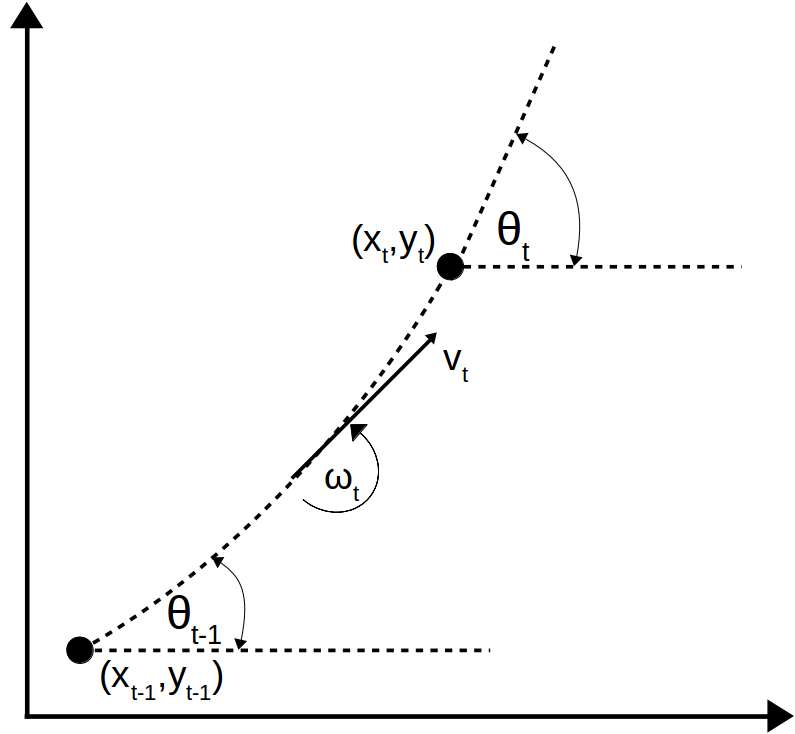
\includegraphics[width=0.4\linewidth]{Figures/velocity_model.png}
  \centering
  \caption{Velocity motion model}
  \label{fig:vel_model}
\end{figure}

Positive rotational velocities are defined to be counterclockwise and positive translational velocities are specified to be in the "forward" direction.
The pose at time $t$ can be determined by
\begin{equation}
\begin{bmatrix}
x_t\\
y_t\\
\theta_t
\end{bmatrix}
=
\begin{bmatrix}
x_{t-1} - \frac{v_t}{\omega_t} \sin\theta_{t-1} + \frac{v_t}{\omega_t} \sin(\theta_{t-1} + \omega_t \Delta t)\\
y_{t-1} + \frac{v_t}{\omega_t} \cos\theta_{t-1} - \frac{v_t}{\omega_t} \cos(\theta_{t-1} + \omega_t \Delta t)\\
\theta_{t-1} + \omega_t \Delta t
\end{bmatrix}+
\begin{bmatrix}
\varepsilon_x\\
\varepsilon_y\\
\varepsilon_\theta\\
\end{bmatrix},
\end{equation}
where
\begin{equation}
\varepsilon_x \sim \mathcal{N}(\varepsilon_x; 0, {\sigma_x}^2),
\end{equation}
\begin{equation}
\varepsilon_y \sim \mathcal{N}(\varepsilon_y; 0, {\sigma_y}^2)
\end{equation}
and
\begin{equation}
\varepsilon_\theta \sim \mathcal{N}(\varepsilon_\theta; 0, {\sigma_\theta}^2),
\end{equation}
and where variances ${\sigma_x}^2$, ${\sigma_y}^2$ and ${\sigma_\theta}^2$ are determined empirically.

The model is nonlinear due to the fact that the movement of the robot cannot be described by a linear translation in the form of
\begin{equation}
\bm{y} = A\bm{x} + B.
\end{equation}

The motion models described in this chapter will be used in subsequent chapters to describe the movement of a robot.
%\chapter{Measurement Models}
%As mentioned in the introduction, measurements retrieved from %sensors always contain noise. A measurement model can be used% %one can describe it with a model. This chapter will describe %the linear measurement model and is based on Thrun~%%\citep{thrun}.
%\section{Linear Measurement Model}
\chapter{Localisation using Kalman Filters}\label{chap:kalmanFilter}
This chapter will focus on estimating the location of a robot, using traditional estimators namely, the Kalman filter, the extended Kalman filter (EKF) and the unscented Kalman filter (UKF). The general theory of the EKF and UKF are discussed in terms of both nonlinear movement and measurements, but when the estimators are applied in Python code, only nonlinear movement is considered while measurements are assumed to be linear. One should pay close attention to the Bayes filter as discussed in Section \ref{sec:bayesFilter}, because all subsequent estimators discussed, are variations of the Bayes filter. The operations of the Bayes filter are also similar to a PGM which is modelled in Chapter \ref{chap:pgmLoc}. This chapter is based on the work of Thrun~\citep{thrun}. 

\section{Background}
A concept that is often used is in this report is that of \textit{belief}. As mentioned in the introduction, a robot cannot know its exact pose. A robot can infer a belief or can have an internal knowledge of its state from information obtained from the sensors. There is thus a difference between internal belief and true state.

In this report the belief, also known as the posterior, is the conditional probability distribution (CPD) of a state variable $\bm{x}_t$ given that all the previous measurements $\bm{z}_{1:t}$ and controls $\bm{u}_{1:t}$ are known. The belief of a state variable is denoted as
\begin{equation}
\bm{x}_t \sim bel(\bm{x}_t),
\end{equation}
which is a reduced notation for the posterior
\begin{equation}
bel(\bm{x}_t) = p(\bm{x}_t| \bm{z}_{1:t}, \bm{u}_{1:t}).
\end{equation}
The belief $bel(\bm{x}_t)$ is usually calculated from a \textit{predicted belief} $\overline{bel}(\bm{x}_t)$. This calculation step is known as the \textit{measurement update}.

The \textit{predicted belief} is defined as
\begin{equation}
\overline{bel}(\bm{x}_t) = p(\bm{x}_t|\bm{z}_{1:t-1}, \bm{u}_{1:t}),
\end{equation} 
and is the CPD of the state variable $\bm{x}_t$ without taking the measurement $\bm{z}_t$ into consideration.
\section{Bayes Filter}\label{sec:bayesFilter}
The \textit{Bayes Filter} algorithm is the generic cornerstone for determining beliefs and is covered to understand the principle on which subsequent estimators work. Algorithm \ref{bayesAlg} shows the general process of the Bayes filter which is recursive as the belief $bel(\bm{x}_{t})$ at the time $t$ is determined from the previous belief $bel(\bm{x}_{t-1})$ at the time $t-1$. The algorithm receives and uses the previous belief $bel(\bm{x}_{t-1})$, the latest control input $\bm{u}_t$ and the measurements $\bm{z}_t$ to calculate the belief $bel(\bm{x}_t)$. Algorithm \ref{bayesAlg} shows one iteration of the process which consists of two steps, namely the \textit{prediction} step in line 3, and \textit{measurement update} step in line 4.

The prediction step calculates a predicted belief of the state $\bm{x}_t$ based on the belief of the previous state $\bm{x}_{t-1}$ and the current control input $\bm{u}_t$.

In the \textit{measurement update} step, the final belief of state $\bm{x}_t$ is calculated by multiplying the predicted belief $\overline{bel}(\bm{x}_t)$ by the probability that $\bm{z}_t$ is observed. The result is usually not a valid PDF and has to be normalized by multiplying it with a normalisation constant, $\eta$. Lastly in line 6, the final belief $bel(\bm{x}_t)$ at time $t$ is returned.
\begin{algorithm}
\caption{Bayes Filter}\label{bayesAlg}
\begin{algorithmic}[1]
\Procedure{Bayes\_Filter}{$bel(\bm{x}_{t-1}), \bm{u}_t, \bm{z}_t$}
\ForAll{$\bm{x}_t$}
\State $\overline{bel}(\bm{x}_t) = \int p(\bm{x}_t|\bm{u}_t, \bm{x}_{t-1})bel(\bm{x}_{t-1})\, d\bm{x}_{t-1}$
\State $bel(\bm{x}_t) = \eta p(\bm{z}_t|\bm{x}_t) \overline{bel} (\bm{x}_t)$
\EndFor
\State \textbf{return} $bel(\bm{x}_t)$
\EndProcedure
\end{algorithmic}
\end{algorithm}

\section{Kalman Filter}
The Kalman filter is an variation of the Bayes filter and is used for prediction in linear Gaussian systems. The Kalman filter is used for the belief estimation of systems with continuous states and is not applicable in discrete state spaces. 
\subsection{Description of the Kalman Filter}
The Kalman filter makes three assumptions in addition to the Markov assumptions. The outcome of this is that each belief $bel(\bm{x}_t)$, which is calculated with the Kalman filter, is a Gaussian distribution.

The three assumptions are as follows:

1. Linear system dynamics are assumed. The motion model describing the movement must be linear, with Gaussian noise $\bm{\varepsilon}$ added, and it must be possible to express it in the form of
\begin{equation}\label{eq:linearKmm}
\bm{x}_t = A_t \bm{x}_{t - 1} + B_t \bm{u}_t + \bm{\varepsilon}_t,
\end{equation}
where the noise $\bm{\varepsilon}_t$ is described by 
\begin{equation}
\bm{\varepsilon}_t \sim \mathcal{N}(\bm{\varepsilon}_t; \bm{0}, R_t).
\end{equation}
The arguments of the state transition CPD, $p(\bm{x}_t|\bm{u}_t, \bm{x}_{t-1})$, can therefore be described by a linear function.

2. Linear measurements with Gaussian noise $\bm{\zeta}_t$ are assumed. The measurement PDF $p(\bm{z}_t|\bm{x}_t)$ is thus also linear in its arguments and can be described by
\begin{equation}
\bm{z}_t = C_t \bm{x}_t + \bm{\zeta}_t,
\end{equation} 
where the noise $\bm{\zeta}_t$ is described by
\begin{equation}\label{eq:linearMeasurements}
\bm{\zeta}_t \sim \mathcal{N}(\bm{\zeta}_t; \bm{0}, Q_t).
\end{equation}

3. Lastly it is assumed that the initial belief $bel(\bm{x}_0)$ of the system is a Gaussian distribution.

The process for the Kalman filter is shown in Algorithm \ref{alg:kalmanFilter}. It is a variation of the Bayes filter and therefore the same principle is followed as in Algorithm \ref{bayesAlg}. The algorithm receives the parameters, $\bm{\mu}_{t-1}$ and $\Sigma_{t-1}$, of the previous belief $bel(\bm{x}_t)$, along with the control vector $\bm{u}_t$ and measurement vector $\bm{z}_t$. In line 2 the previous mean $\bm{\mu}_t$ is transformed through the linear state transition function to determine the predicted mean $\overline{\bm{\mu}}_t$ of the predicted belief. In line 3 the covariance $\Sigma_{t-1}$ is multiplied twice with $A_t$, then $R_t$ is added to determine the predicted covariance $\overline{\Sigma}_t$ of the predicted belief. Lines 2 and 3 therefore contain the \textit{prediction} step of the Bayes filter where the predicted belief $\overline{bel}(x_t)$ is calculated. 

Lines 4 to 6 correspond with the \textit{measurement update} step of the Bayes filter in which the mean $\bm{u}_t$ and the covariance $\Sigma_t $ of the the desired belief $bel(\bm{x}_t)$ is computed. The Kalman gain $K_t$ is calculated in line 4 and is used to determine how much influence the measurement $\bm{z}_t$ has when it is incorporated. The difference between the actual measurement $\bm{z}_t$ and the expected measurement $C_t \bm{\overline{\mu}}_t$ is called the innovation. In line 5 the predicted mean $\overline{\bm{\mu}}_t$ is adjusted by adding it to the product of the Kalman gain and the innovation. In line 6 the covariance $\Sigma_t$ of the posterior belief $bel(\bm{x}_t)$ is calculated by adjusting the predicted covariance $\overline{\Sigma}_t$. 
\begin{algorithm}
\caption{Kalman Filter}\label{alg:kalmanFilter}
\begin{algorithmic}[1]
\Procedure{Kalman\_Filter}{$\bm{\mu}_{t-1}, \Sigma_{t-1},\bm{u}_t, \bm{z}_t$}
\State $\overline{\bm{\mu}}_t = A_t \bm{\mu}_{t-1} + B_t \bm{u_}t$
\State $\overline{\Sigma}_t = A_t \Sigma_{t-1} A_t^T + R_t$
\State $K_t = \overline{\Sigma}_t C_t^T(C_t\overline{\Sigma}_t C_t^T + Q_t)^{-1}$
\State $\bm{\mu}_t = \overline{\bm{\mu}}_t + K_t(\bm{z}_t - C_t \overline{\bm{\mu}}_t)$
\State $\Sigma_t = (I - K_tC_t)\overline{\Sigma}_t$
\State \textbf{return} $\bm{\mu}_t, \Sigma_t$
\EndProcedure
\end{algorithmic}
\end{algorithm}

\subsection{Application of the Kalman Filter}\label{subsec:appEKF}
The Kalman filter is applied to determine the belief of the location of a linear moving robot. A moving robot is simulated and the Kalman filter (Algorithm \ref{alg:kalmanFilter}) is implemented in Python to find the belief $bel(\bm{x}_t)$ at each time step $t$.

The movement of the robot is described by the linear motion model in Section \ref{sec:linearMotionModel} by Equation \ref{eq:lineartrans},
where the matrix A is specified as
\begin{equation}
A =
\begin{bmatrix}
1 & 0\\
0 & 1
\end{bmatrix},
\end{equation}
the matrix $B$ is specified
\begin{equation}
B =
\begin{bmatrix}
\Delta t & 0\\
0 & \Delta t
\end{bmatrix}, \Delta t = 1,
\end{equation}
and the covariance $R_t$ is specified as
\begin{equation}
R_t =
\begin{bmatrix}
0.1 & 0\\
0 & 0.1
\end{bmatrix}.
\end{equation}
Measurements are linear with Gaussian noise as required in Equation \ref{eq:linearMeasurements},
with the covariance matrix $Q_t$ specified as
\begin{equation}
Q_t =
\begin{bmatrix}
0.1 & 0\\
0 & 0.1
\end{bmatrix}.
\end{equation}
The initial belief $bel(\bm{x}_0)$ of the robot's location is known and five control commands in the form of a list is given to the robot. At each time step the controls and measurements are given to the Kalman filter, which produces the belief of the robot's state at time $t$. The result of the simulation is shown in Figure \ref{fig:resultKF}, where the purple error ellipses indicate the 95\% confidence level region of each belief $bel(\bm{x}_t)$. The purple dots indicate the mean of each belief $bel(\bm{x}_t)$ at time $t$. The exact position of the robot at each time step is indicated with a black cross.

\begin{figure}[H]

  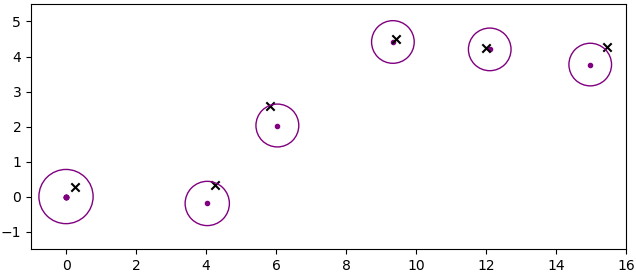
\includegraphics[width=0.8\linewidth]{Figures/result_kalmanfilter.png}
  \centering
  \caption{Result of application with Kalman filter}
  \label{fig:resultKF}
\end{figure}

\section{Extended Kalman Filter}
The Kalman filter as discussed above is very efficient due to the fact that state transitions and measurements are assumed to be linear, hence the mean $\bm{\mu}_t$ and covariance $\Sigma_t$ of a resulting belief $bel(\bm{x}_t)$ can be computed analytically.
As mentioned in Chapter \ref{chap:motionModel}, state transitions and measurements are in practice seldom linear and therefore the normal Kalman filter is not suitable for most robotics problems. 

\subsection{Description of EKF}
The extended Kalman filter (EKF) lifts the constraint of linear state transition and measurement functions. These functions are now described in a more general form. The state transition of a nonlinear system can be described by
\begin{equation}
\bm{x}_t = \bm{g}(\bm{u}_t, \bm{x}_{t-1}) + \bm{\varepsilon}_t,
\end{equation}
and the nonlinear measurements can be described by
\begin{equation}
\bm{z}_t = \bm{h}(\bm{x}_t) + \bm{\zeta}_t,
\end{equation}
where $\bm{h}$ and $\bm{g}$ are nonlinear vector functions. If one performs a nonlinear transformation on a Gaussian random variable (RV), it will result in a non-Gaussian RV. Therefore, if the state transition or measurement functions of a system are nonlinear, the belief $bel(\bm{x}_t)$ will not be a Gaussian distribution and cannot be computed analytically.

The extended Kalman filter (EKF) is a variation of the Kalman filter and enables one to approximate the belief $bel({\bm{x}_t})$ of a nonlinear system as a Gaussian distribution. The EKF accomplishes this by using Taylor expansion to linearise the functions $\bm{h}$ and $\bm{g}$.

In general, with Taylor expansion a nonlinear vector function
\begin{equation}
\bm{f}(\bm{x}) =
\begin{bmatrix}
f_1(\bm{x}) & ... & f_M(\bm{x})
\end{bmatrix}^T,
\end{equation}
where the vector $\bm{x}$ is defined as
\begin{equation}
\bm{x} =
\begin{bmatrix}
x_1 & ... & x_N
\end{bmatrix}^T,
\end{equation}
can be approximated as a linear vector function that is tangent to a given point $\bm{k}$ 
\begin{equation}\label{eq:taylorGeneral}
\bm{f}(\bm{x}) \approx \bm{f}(\bm{k}) + \bm{f}'(\bm{k})(\bm{x-k}),
\end{equation}
where $\bm{f}'(\bm{x})$ is the Jacobian matrix and is calculated as
\begin{equation}\label{eq:jacobian}
\bm{f}'(\bm{x}) = \frac{\partial\bm{f}(\bm{x})}{\partial \bm{x}} =
\begin{bmatrix}
\frac{\partial f_1}{\partial x_1} & \dots &\frac{\partial f_1}{\partial x_N}\\
\vdots & \ddots &\vdots\\
\frac{\partial f_M}{\partial x_1} & \dots &\frac{\partial f_M}{\partial x_N}
\end{bmatrix}.
\end{equation}
Taylor expansion can now be applied to linearise the nonlinear vector functions $\bm{g}$ and $\bm{h}$. The function $\bm{g}$ can be approximated as a linear vector function around $\bm{\mu}_{t-1}$ by means of Equation \ref{eq:taylorGeneral}
\begin{equation}\label{eq:linear_taylor}
\begin{split}
\bm{g}(\bm{u_t}, \bm{x}_{t-1}) & \approx \bm{g}(\bm{u}_t, \bm{\mu}_{t-1}) + \bm{g}'(\bm{u}_t, \bm{\mu}_{t-1})(\bm{x}_{t-1} - \bm{\mu}_{t-1})\\
& = \bm{g}(\bm{u}_t, \bm{\mu}_{t-1}) + G_t(\bm{x}_{t-1} - 
\bm{\mu}_{t-1}),
\end{split}  
\end{equation}
where $G_t$ is the Jacobian matrix and can be determined with Equation \ref{eq:jacobian}, therefore
\begin{equation}\label{eq:Gt}
G_t = \bm{g}'(\bm{u}_t, \bm{\mu}_{t-1}) = \frac{\partial \bm{g}(\bm{u}_t, \bm{x}_{t-1})}{\partial \bm{x}_{t-1}}.
\end{equation}
The same procedure can be followed to approximate the measurement function $\bm{h}$ as a linear vector function around the predicted mean $\overline{\bm{\mu}}$
\begin{equation}
\begin{split}
\bm{h}(\bm{x}_{t}) & \approx \bm{h}(\bm{\overline{\mu}}_{t}) + \bm{h}'(\bm{\overline{u}}_t)(\bm{x}_{t} - \bm{\overline{\mu}}_{t})\\
& = \bm{h}(\bm{\overline{\mu}}_t) + H_t(\bm{x}_{t} - 
\bm{\overline{\mu}}_{t}),
\end{split}  
\end{equation}
where
\begin{equation}\label{eq:Ht}
H_t = \bm{h}'(\bm{u}_t) = \frac{\partial \bm{h}(\bm{x}_{t})}{\partial \bm{x}_{t}}.
\end{equation}
In Algorithm \ref{alg:EKF} the procedure of the EKF is shown and one will notice that it is very similar to Algorithm \ref{alg:kalmanFilter} of the Kalman filter. It can be seen that $G_t$ and $H_t$ in Algorithm \ref{alg:EKF} are respectively equivalent to $A_t$ and $C_t$ in Algorithm \ref{alg:kalmanFilter}. It must also be remembered that the nonlinear functions are approximated as linear functions, therefore the belief computed by the EKF is only an approximated belief and not the ground truth.

\begin{algorithm}
\caption{Extended Kalman Filter}\label{alg:EKF}
\begin{algorithmic}[1]
\Procedure{EKF}{$\bm{\mu}_{t-1}, \Sigma_{t-1},\bm{u}_t, \bm{z}_t$}
\State $\overline{\bm{\mu}}_t = \bm{g}(\bm{u}_t, \bm{\mu}_{t-1})$
\State $\overline{\Sigma}_t = G_t \Sigma_{t-1} G_t^T + R_t$
\State $K_t = \overline{\Sigma}_t H_t^T(H_t\overline{\Sigma}_t H_t^T + Q_t)^{-1}$
\State $\bm{\mu}_t = \overline{\bm{\mu}}_t + K_t(\bm{z}_t - h(\overline{\bm{\mu}}_t))$
\State $\Sigma_t = (I - K_tH_t)\overline{\Sigma}_t$
\State \textbf{return} $\bm{\mu}_t, \Sigma_t$
\EndProcedure
\end{algorithmic}
\end{algorithm}
This section covers the basic theory of the EKF, and the next section will discuss how the EKF can be applied to estimate the belief of a nonlinear system.
\subsection{Application of EKF}
In this subsection the EKF is applied to estimate the location of a robot which movement is described by the velocity motion model.

The robot's pose $\bm{x}_t$ at time $t$ is dependent on the previous pose $\bm{x}_{t-1}$ at time $t-1$ and the control $\bm{u}_t$. The transition of the robot's pose can be described in general as
\begin{equation}\label{eq:stateTranGen}
\bm{x}_t =
\begin{bmatrix}
x_t\\
y_t\\
\theta_t
\end{bmatrix}
= \bm{g}(\bm{u}_t, \bm{x}_{t-1}) + \bm{\varepsilon}_t,
\end{equation}
where $\bm{g}$ is described by the velocity motion model as
\begin{equation}
\bm{g}(\bm{u}_t, \bm{x}_{t-1})=
\begin{bmatrix}
x_{t-1} - \frac{v_t}{\omega_t} \sin\theta_{t-1} + \frac{v_t}{\omega_t} \sin(\theta_{t-1} + \omega_t \Delta t)\\
y_{t-1} + \frac{v_t}{\omega_t} \cos\theta_{t-1} - \frac{v_t}{\omega_t} \cos(\theta_{t-1} + \omega_t \Delta t)\\
\theta_{t-1} + \omega_t \Delta t
\end{bmatrix}.
\end{equation}
The noise $\bm{\varepsilon}$ is defined as
\begin{equation}
\bm{\varepsilon_t} \sim \mathcal{N}(\bm{\varepsilon_t}; \bm{0}; R_t),
\end{equation}
where the covariance matrix R is defined as
\begin{equation}
R_t =
\begin{bmatrix}
\sigma_x^2 & 0 & 0\\
0 & \sigma_y^2 & 0\\
0 & 0 & \sigma_\theta^2
\end{bmatrix}.
\end{equation}
$R_t$ is a diagonal matrix, hence the noise added to each RV is independent.

The next step is to linearise the nonlinear vector function $\bm{g}$ by means of Taylor expansion. Equation \ref{eq:jacobian} and Equation \ref{eq:Gt} can be used to calculate the Jacobian matrix $G_t$ of $\bm{g}$:
\begin{equation}\label{eq:velocityJacobian}
G_t = \bm{g}'(\bm{u}_t, \bm{x}_{t-1}) =
\begin{bmatrix}
1 & 0 & -\frac{v_t}{\omega_t} \cos\theta + \frac{v_t}{\omega_t} \cos(\theta + \omega_t \Delta t)\\
0 & 1 & -\frac{v_t}{\omega_t}\sin\theta + \frac{v_t}{\omega_t}\sin(\theta + \omega_t \Delta t)\\
0 & 0 & 1 
\end{bmatrix}.
\end{equation}
Using Equation \ref{eq:linear_taylor} and the Jacobian matrix $G_t$ calculated in Equation \ref{eq:velocityJacobian}, the vector function $\bm{g}$ can be linearised around $\bm{u_{t-1}}$, thus
\begin{equation}\label{eq:linearG}
\bm{g}(\bm{u_t}, \bm{x}_{t-1}) \approx \bm{g}(\bm{u}_t, \bm{\mu}_{t-1}) + G_t(\bm{x}_{t-1} - 
\bm{\mu}_{t-1}).
\end{equation} 
Using the result in Equation \ref{eq:linearG}, the state transition in Equation \ref{eq:stateTranGen} can be approximated as
\begin{equation}
\bm{x}_t \approx \bm{g}(\bm{u}_t, \bm{\mu}_{t-1}) + G_t(\bm{x}_{t-1} - \bm{\mu}_{t-1}) + \bm{\varepsilon}.
\end{equation} 
Linear measurements are assumed for this application and therefore we can use Equation \ref{eq:linearMeasurements} to describe $\bm{z}_t$,
where
\begin{equation}
C_t = 
\begin{bmatrix}
1 & 0\\
0 & 1
\end{bmatrix}
\end{equation}

Five time steps of the movement of a robot were simulated in Python. The initial belief of the robot is known and five control inputs are given to the robot in by means of a list. Algorithm \ref{alg:EKF}, tailored for the velocity motion model, is implemented and the result of the application can be seen in Figure \ref{fig:resultEKF}. The green ellipses represent the 95\% confidence region and the green dots represent the mean of each belief $bel(\bm{x}_t)$ at time $t$. The exact position of the robot of each time step $t$ is represented by the black cross.

\begin{figure}[H]
  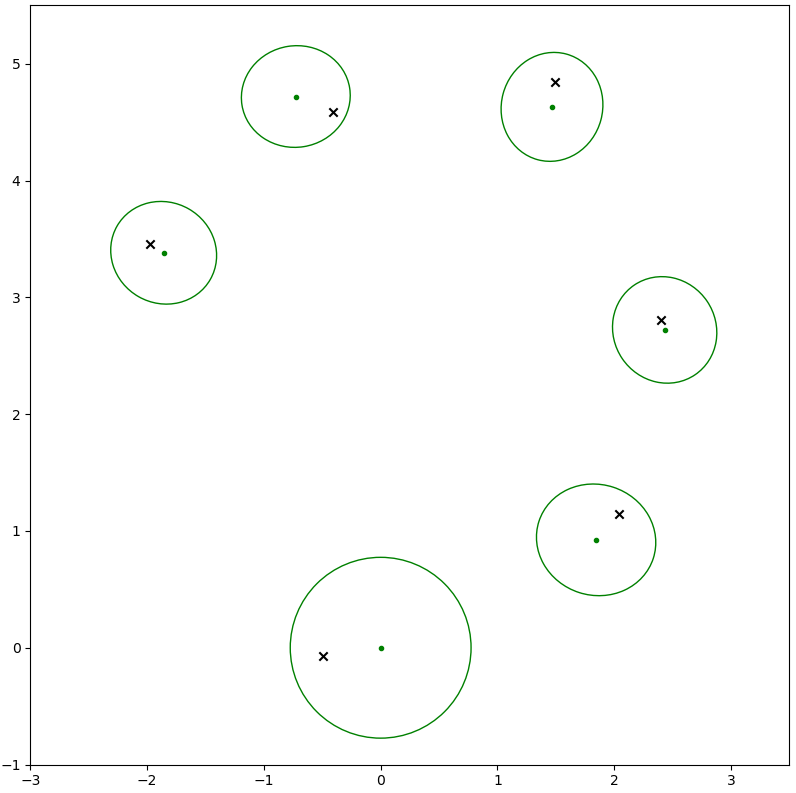
\includegraphics[width=0.7\linewidth]{Figures/result_EKF.png}
  \centering
  \caption{Result of the application of the extended Kalman filter}
  \label{fig:resultEKF}
\end{figure}

\section{Unscented Kalman Filter}\label{sec:UKF}
The linearisation used in the EKF can sometimes be very inaccurate, as the nonlinear functions are linearised only around the mean $\bm{u}_t$. The unscented Kalman filter (UKF) is an alternative approach which in many cases deliver better results than that of the EKF, especially when $\bm{g}$ and $\bm{h}$ are severely nonlinear.

As mentioned before, a Gaussian distribution that is transformed through a nonlinear function results in a distribution that is not Gaussian. The principle on which UKF is based, is to draw carefully chosen points called \textit{sigma points} around the mean of an existing Gaussian distribution and transform them through a nonlinear function. The transformed sigma points can then be used to approximate the resultant distribution as a Gaussian distribution.

Usually one sigma point is located at the mean and for each dimension two sigma points are located symmetrically around the mean along the main axes. For an $n$-dimensional Gaussian distribution, there are $2n +1$ sigma points selected. Sigma points are denoted as
\begin{equation}
\mathcal{X}^{[i]},\ i\ = \ 0,\ ...,\ 2n,
\end{equation}
where $i$ indicates the index of the sigma point.

Sigma points are determined as follows:
\begin{flalign}
    &\mathcal{X}^{[0]} = \bm{\mu},& \\
    &\mathcal{X}^{[i]} = \bm{\mu} + \left(\sqrt{(n + \lambda)\Sigma}\right)\ \text{for}\ \ i =1, ...,n,&\\ 
    &\mathcal{X}^{[i]} = \bm{\mu} - \left(\sqrt{(n + \lambda)\Sigma}\right)\ \text{for}\ \ i = n + 1, ...,2n,&
\end{flalign}
where the scaling parameter $\lambda$ is defined as
\begin{equation}\label{eq:calcLam}
\lambda = \alpha^2(n+\kappa) - n.
\end{equation}
The parameters $\alpha$ and $\kappa$ determines the spread of the sigma points around the mean.

Each sigma point $\mathcal{X}^{[i]}$ has corresponding weights $w_m^{[i]}$  and $w_c^{[i]}$, which are respectively used to recover the mean $\bm{\mu}_t$ and covariance $\Sigma_t$. Weights corresponding to the sigma point $\mathcal{X}^{[0]}$ are determined as 
\begin{flalign}
    &w_m^{[0]} = \frac{\lambda}{n + \lambda},& \\ 
    &w_c^{[0]} = \frac{\lambda}{n+\lambda} + (1 - \alpha^2 + \beta).&
\end{flalign}
The optimal choice for the parameter $\beta$ is normally 2.
The rest of the weights ($i = 1\ ,...,\ 2n$) are determined as
\begin{flalign}
    &w_m^{[i]} = w_c^{[i]} = \frac{1}{2(n + \lambda)}\ \ \text{for}\ i=1,\ ...,\ 2n.& 
\end{flalign}
After sigma points and weights have been calculated, the chosen sigma points can be transformed through a nonlinear vector function $\bm{f}$ to determine the resulting sigma points $\mathcal{Y}^{[i]}$ given by 
\begin{equation}
\mathcal{Y}^{[i]} = \bm{f}\left(\mathcal{X}^{[i]}\right).
\end{equation}
The distribution as a result of the nonlinear transformation can be approximated as a Gaussian distribution by estimating the mean $\bm{u}_{\bm{y}}$ and covariance $\Sigma_{\bm{yy}}$ with 
\begin{equation}\label{eq:unscentedMean}
\bm{\mu}_{\bm{y}} = \sum_{i = 0}^{2n}w_m^{[i]}\mathcal{Y}^{[i]},
\end{equation}
\begin{equation}\label{eq:unscentedCov}
\Sigma_{\bm{yy}} = \sum_{i=0}^{2n}w_c^{[i]}\left(\mathcal{Y}^{[i]} \right)
\end{equation}
The procedure of the UKF is shown in Algorithm \ref{alg:UKF}. Lines 1 to 5 relates to the \textit{prediction} step of the Bayes filter. Sigma points are deterministically selected in line 2 and passed through the nonlinear function $\bm{g}$ in line 3. The parameters of the predicted belief $\overline{bel}(\bm{x}_t)$ are computed in lines 4 and 5. Lines 6 to 13 correspond to the \textit{measurement update} step of the Bayes filter. In line 6, the predicted mean $\overline{\bm{\mu}}_t$ and covariance matrix $\overline{\Sigma}_t$ are used to extract new sigma points $\overline{\mathcal{X}}_t$. The predicted measurement for each sigma point is determined in line 7. The resulting sigma points $\overline{\mathcal{Z}}$ are used in lines 8 and 9 to calculate the mean $\hat{\bm{z}}_t$ and covariance $S_t$ of the predicted measurement. In line 10 the cross covariance $\overline{\Sigma}_t^{\bm{x,z}}$ is calculated and in line 11 the Kalman gain $K_t$ is determined. In lines 12 and 13 the updated parameters, $\bm{\mu}_t$ and $\Sigma_t$, of the belief $bel(\bm{x}_t)$ are calculated.
\begin{algorithm}
\caption{Unscented Kalman Filter}\label{alg:UKF}
\begin{algorithmic}[1]
\Procedure{UKF}{$\bm{\mu}_{t-1}, \Sigma_{t-1},\bm{u}_t, \bm{z}_t$}
\State $\mathcal{X}_{t-1} = 
\begin{pmatrix}
\bm{\mu}_{t-1}  & \ \bm{\mu}_{t-1}+\sqrt{(n + \lambda)\Sigma_{t-1}} & \ \bm{\mu}_{t-1} - \sqrt{(n + \lambda)\Sigma_{t-1}}\ \ 
\end{pmatrix}
$ 
\State $\overline{\mathcal{X}}^*_{t-1} = \bm{g}(\bm{u}_t, \mathcal{X}_{t-1})$
\State $\bm{\overline{\mu}}_t = \sum_i^{2n} w_m^{[i]} \overline{\mathcal{X}}^{*[i]}_{t}$
\State $\overline{\Sigma}_t = \sum_i^{2n}w_c^{[i]}\left(\mathcal{\overline{X}}_t^{*[i]} - \overline{\bm{\mu}}_t\right)\left(\mathcal{\overline{X}}_t^{*[i]} - \overline{\bm{\mu}}_t\right)^T +R_t$
\State $\mathcal{\overline{X}}_t = 
\begin{pmatrix}
\bm{\overline{\mu}}_{t}  & \ \bm{\overline{\mu}}_{t}+\sqrt{(n + \lambda)\overline{\Sigma}_{t}} & \ \bm{\overline{\mu}}_{t} -  \sqrt{(n + \lambda)\overline{\Sigma}_{t}}\ \ 
\end{pmatrix}$
\State $\overline{\mathcal{Z}}_t = \bm{h}\left(\mathcal{\overline{X}}_t\right)$
\State $\hat{\bm{z}}_t = \sum_{i=0}^{2n}w_m^{[i]} \overline{\mathcal{Z}}_t^{[i]}$ 
\State $S_t = \sum_{i=0}^{2n} w_c^{[i]}\left( \overline{\mathcal{Z}}_t^{[i]} - \hat{\bm{z}}_t  \right)\left( \overline{\mathcal{Z}}_t^{[i]} - \hat{\bm{z}}_t  \right)^T + Q_t$
\State $\overline{\Sigma}_t^{x,z} = \sum_{i=0}^{2n}  w_c^{[i]}\left( \overline{\mathcal{X}}_t^{[i]} - \overline{\bm{\mu}}_t  \right)\left( \overline{\mathcal{Z}}_t^{[i]} - \hat{\bm{z}}_t  \right)^T $
\State $K_t = \overline{\Sigma}_t^{x,z}S_t^{-1}$
\State $\bm{\mu}_t = \overline{\bm{\mu}}_t + K_t(\bm{z}_t - \hat{\bm{z}}_t)$
\State $\Sigma_t = \overline{\Sigma}_t - K_tS_tK_t^T$
\State \textbf{return} $\bm{\mu}_t, \Sigma_t$
\EndProcedure
\end{algorithmic}
\end{algorithm}

The general theory of the UKF is covered in this section, the next section will discuss the application of the UKF.
\subsection{Application of UKF}
The unscented Kalman filter (UKF) is applied to solve the same localisation problem as the one given to the EKF in Subsection \ref{subsec:appEKF}. An advantage of using the UKF is that it is not necessary to determine a Jacobian matrix of the transition or measurement functions beforehand. The UKF is therefore generic and suitable for a wide range of problems, where as in the case of the EKF, it is not always possible to calculate the Jacobian matrix of a function.

For this application of the UKF the parameter $\lambda$ is defined as
\begin{equation}
\lambda = n - 1,
\end{equation}
where $n$ is the length of the state vector $\bm{x}_t$. The parameter $\kappa$ is set to 0 and the parameter $\alpha$ can then be obtained from Equation \ref{eq:calcLam}. Finally, $\beta$ is set to 2.

Algorithm \ref{alg:UKF} is implemented in Python to estimate the belief of the state $\bm{x}_t$ of the robot at time $t$.  At each time step the controls, noisy measurements and the previous belief $bel(\bm{x}_{t-1})$ are given to the UKF, which produces the belief of the robot's state at time $t$. The result can be viewed in Figure \ref{fig:resultUKF}, where the blue error ellipses indicate the 95\% confidence level region of each belief $bel(\bm{x}_t)$. The blue dots indicate the mean of each belief $bel(\bm{x}_t)$ at time $t$. The precise position of the robot at each time step is indicated with a black cross.


\begin{figure}[H]
  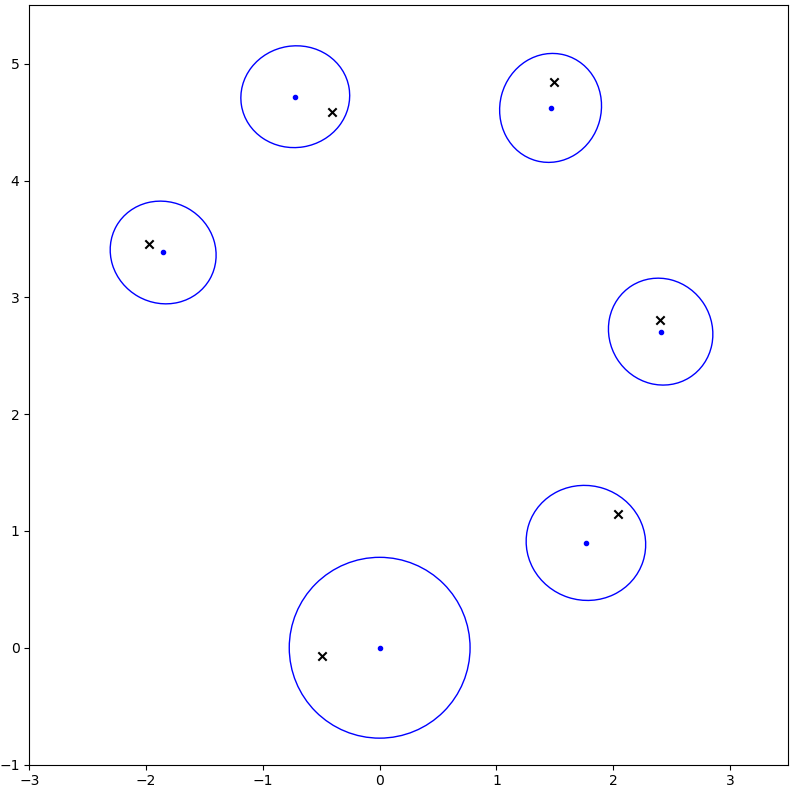
\includegraphics[width=0.7\linewidth]{Figures/result_UKF.png}
  \centering
  \caption{Result of the application of the unscented Kalman filter}
  \label{fig:resultUKF}
\end{figure}

\chapter{Probabilistic Graphical Models}
This chapter gives a brief introduction to the probabilistic graphical models which will be used to solve the localisation problem, using different techniques of numerical integration. PGMs form part of a vast study field, therefore only the theory relevant to this report will be discussed. This chapter is based on the work of Koller and Friedman~\cite{koller}, Barber~\cite{barber} and Schoeman~\citep{JC}.
\section{Overview}
Reasoning about systems that have a measure of uncertainty can become very complex. Sometimes these systems are completely unmanageable. The PGM is a graphical technique which makes problems tractable by modelling probabilistic systems in a logical and compact manner. PGMs are thus used to describe the relationship between variables and allow one to reason about it. The querying of a system or reasoning about a variable is called inference. It is a very popular technique, as it is intuitive, transparent and easy to manipulate. Hence, PGMs have countless applications from diagnosing medical problems to estimating the location of a robot.

PGMs used for modelling can be divided into two categories. The first includes Markov networks, which are used for non-causal systems. The second includes Bayesian networks, where relationships between random variables are causal and specified as CPDs. As the localisation problem in most cases is causal, the focus of this chapter is on Bayesian networks. Due to the relevance to localisation, the theory is discussed in terms of continuous random variables, but it can also be applied to discrete random variables. 
\section{Basic Concepts of Graphical Models}
There are a few basic concepts to understand before defining a Bayesian network. Graphical models consist of nodes and edges. Edges are the links between nodes and can be directed or undirected. A Markov network is described by an undirected graph, where all edges are undirected. A Bayesian network is described by a directed graph, where all the edges are directed. An example of an undirected and directed graph can be seen in Figure \ref{fig:undirected_graph} and Figure \ref{fig:directed_graph} respectively.

In the case of directed graphs, nodes can be classified as ancestors, parents, children and descendants. If there exists a directed path from $x_1 \to x_k$, then $x_1$ is an ancestor of $x_k$, and $x_k$ is a descendant of $x_1$. In Figure \ref{fig:directed_graph}, $a$ is an ancestor of $c$ and $c$ is a descendant of $a$. A parent is an ancestor with only one edge between the ancestor and descendant. A child is a descendant with only one edge between the descendant and the ancestor. In Figure \ref{fig:undirected_graph}, $a$ is a parent of $b$ and $b$ is a child of $a$.~\cite{barber}

\begin{figure}[htbp]
  \begin{minipage}[b]{0.5\linewidth}
    \centering
    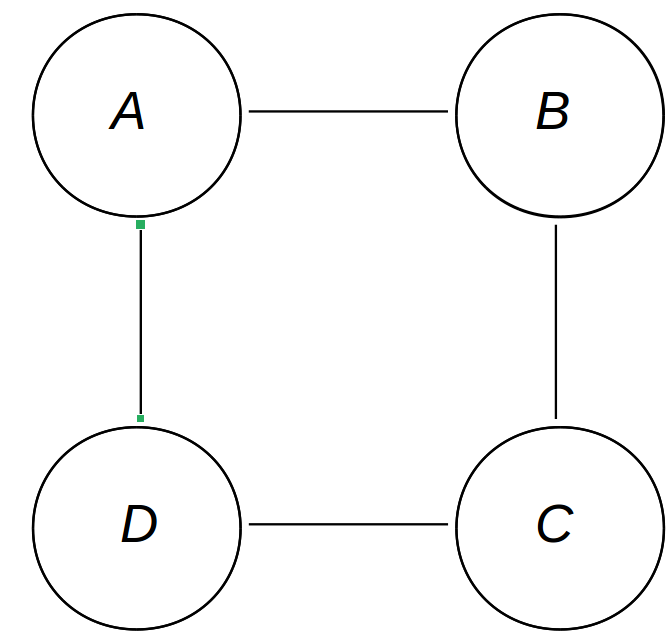
\includegraphics[width=0.5\linewidth]{Figures/undirected_graph.png}
    \caption{Undirected graph}
    \label{fig:undirected_graph}
  \end{minipage}
  \hspace{0.5cm}
  \begin{minipage}[b]{0.5\linewidth}
    \centering
    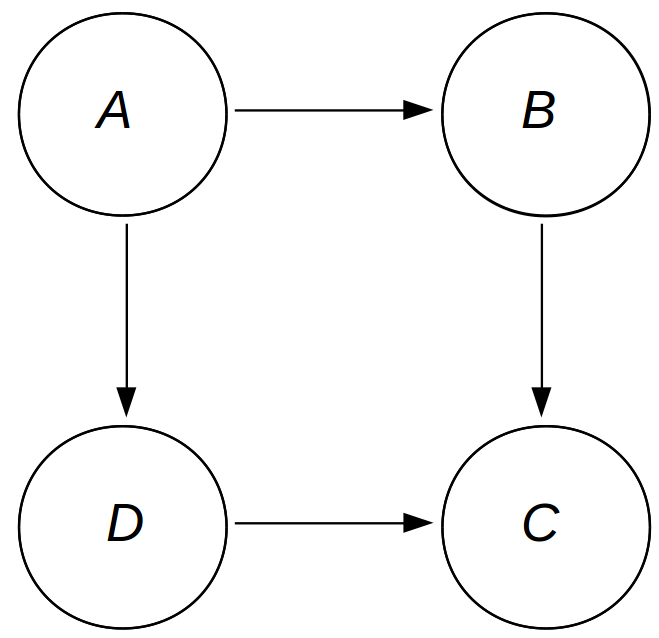
\includegraphics[width=0.5\linewidth]{Figures/directed_graph.png}
    \caption{Directed graph}
    \label{fig:directed_graph}
  \end{minipage}
\end{figure}

\section{Bayesian Networks}
Bayesian networks consists of random variables in the form of nodes and are connected by directed edges. Nodes that are not directly connected to each other, are considered conditionally independent. Relationships between nodes are indicated as conditional probability distributions (CPDs) and each node can be associated with a CPD
\begin{equation}
x_i \sim p(x_i|Par(x_i)),
\end{equation}
where $Par(x_i)$ indicates the parents of node $x_i$.

CPDs can be written as a factors. A factor is a function that takes a number of random variables as arguments and is defined as
\begin{equation}
\phi_i(x_i, Par(x_i)) = p(x_i|Par(x_i)),
\end{equation}
where the scope of a factor is its arguments 
\begin{equation}
\text{Scope}\{\phi_i\} = \{x_i, Par(x_i)\}.
\end{equation}
The concept of a factor is important that will be used in the rest of the report.

Figure \ref{fig:bays_pgm} shows an example of a Bayesian network with seven nodes labelled from $a$ to $g$. Each node is associated with a CPD. Directed edges between nodes are indicated with arrows.
\begin{figure}[H]
  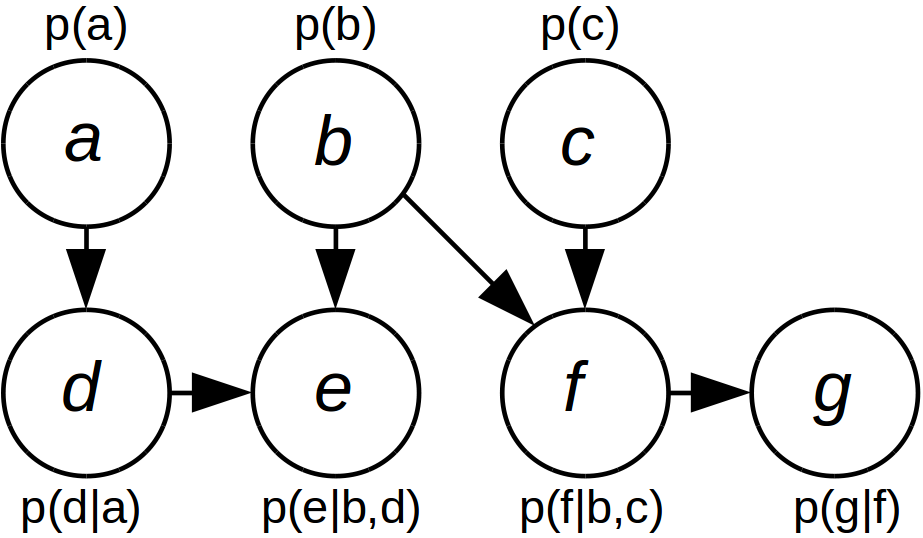
\includegraphics[width=0.5\linewidth]{Figures/bayesian_pgm.png}
  \centering
  \caption{Bayesian network}
  \label{fig:bays_pgm}
\end{figure}
The chain rule specifies that the joint probability density distribution of all the variables in a Bayesian network can be determined by calculating the product of all the CPDs associated with the nodes~\citep{koller}. It is defined as
\begin{equation}
p(x_1, ..., x_n) = \prod_i p(x_i|Par(x_i)).
\end{equation}
The chain rule can be applied to the Bayesian network in Figure \ref{fig:bays_pgm}
\begin{equation}
p(a,b,c,d,e,f,g) = p(a)p(b)p(c)p(d|a)p(e|b,d)p(f|b,c)p(g|f)
\end{equation}
A marginal PDF of the subset of variables $a$, $b$ and $c$ can be determined by integrating over all the variables not in the subset, therefore
\begin{equation}
p(a,b,c) = \int\int\int\int p(a,b,c,d,e,f,g)dd\,de\,df\,dg.
\end{equation}
The chain rule together with marginalisation can be used to infer a Bayesian network, but it can be very tedious. The next section covers an alternative method to reason about a Bayesian network in a structured manner.
\section{Cluster Graphs}
The next step is to reason about variables of a Bayesian network in a more efficient manner. Various methods can be used to inference a Bayesian network; one method is to construct a cluster graph. The cluster graph consists of clusters connected by undirected edges.

Clusters can be formed by grouping factors together such that each cluster $C_i$ is a subset of the variables of the Bayesian network
\begin{equation}
C_i \subseteq \{x_1, ..., x_n\}.
\end{equation}
The undirected edges between clusters are called sepsets and are responsible for passing messages between clusters. A sepset between two clusters contains information about variables that are common to both clusters. An edge between $C_i$ and cluster $C_j$ is associated with a sepset which contains variables that are common to both $C_i$ and $C_j$ and is defined as
\begin{equation}
S_{i,j} \subseteq C_i \cap C_j.
\end{equation}
There are multiple ways to construct clusters, but it should adhere to two requirements~\citep{koller}:

1. Family preservation requires that every factor in the Bayesian network is accommodated by some cluster.

2. The running intersection property states that there exists an unique path connecting a pair of clusters containing the same variable $x$, and every cluster and sepset along the path also contain $x$. This path allows clusters to share their beliefs of $x$. In other words, for any variable $x$, the set of sepsets and clusters containing $x$ form a tree~\citep{koller}. This prevents feedback loops and thus counters the phenomena where clusters reinforce their own beliefs of variables.

Figure \ref{fig:bays_pgm} is converted into Figure \ref{fig:cluster_bound} where CPDs are replaced with factors and possible cluster boundaries are indicated with dashed rectangles. Note that there are other ways to construct the cluster graph.
\begin{figure}[H]
  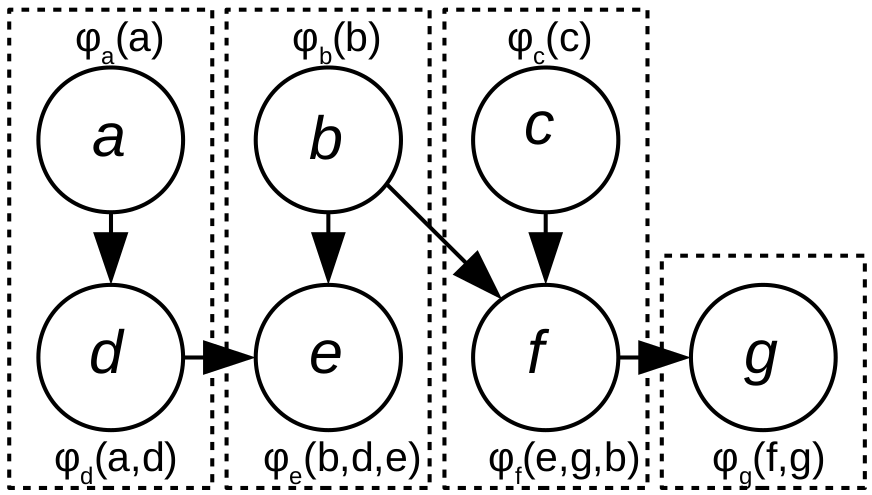
\includegraphics[width=0.6\linewidth]{Figures/cluster_divisions.png}
  \centering
  \caption{Bayesian network with cluster boundaries}
  \label{fig:cluster_bound}
\end{figure}

The cluster factor $\psi_i$ can be calculated by finding the product of all the factors inside the cluster~\citep{koller} and is therefore defined as
\begin{equation}
\psi_i(C_i) = \prod_{k}\phi_k.
\end{equation}
Figure \ref{fig:cluster_bound} is transformed in Figure \ref{fig:clustergraph}. Clusters are indicated by ellipsis. Initial beliefs are calculated and shown inside the ellipsis. Sepsets are indicated by rectangles.
\begin{figure}[H]
  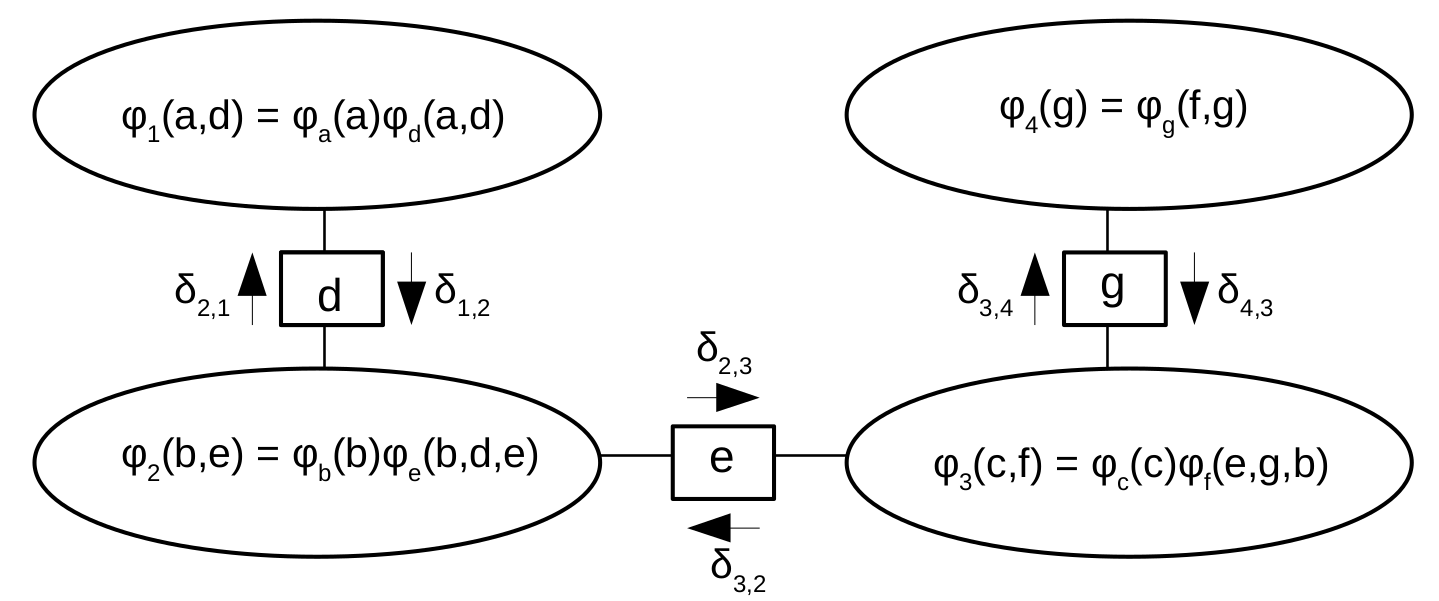
\includegraphics[width=0.7\linewidth]{Figures/clustergraph.png}
  \centering
  \caption{Cluster graph showing sepsets and clusters with initial beliefs}
  \label{fig:clustergraph}
\end{figure}
This section shows how to construct a cluster graph with clusters and sepsets. The cluster graph allows clusters to share beliefs of variables by means of message passing, which will be explored in the next section. 
\section{Message Passing}
Clusters can share beliefs of common variables by using message passing. Every sepset $S_{i,j}$ has two messages, $\delta_{i, j}$ and $\delta_{j,i}$, associated with it. This allows clusters, connected by a sepset, to communicate in both directions. An outgoing message $\delta_{i,j}$ of a cluster $C_i$ can be calculated by multiplying the cluster factor $\psi_i$ with the incoming message $\delta_{k,i}$ from each other cluster $C_k$ and then integrating the result over the variables that are not in the sepset ($C_i - S_{i,j}$). This procedure is defined as~\citep{koller}
\begin{equation}\label{eq:messageOut}
\delta_{i,j}(S_{i,j}) = \int_{C_i - S_{i,j}}\psi_i \times \prod_{k\ne j} \delta_{k,i}(S_{k,i}).
\end{equation}
Equation \ref{eq:messageOut} can be demonstrated by calculating arbitrary messages $\delta_{2,3}$ and $\delta_{3,4}$ in Figure \ref{fig:clustergraph}, therefore
\begin{equation}
\delta_{2,3}(b) = \int_d \int_e \delta_{1,2}(d)\psi_2(b,d,e)dd\ de
\end{equation}
and
\begin{equation}\label{eq:mes34}
\delta_{3,4}(f) = \int_b \int_c \delta_{2,3}(b)\psi_3(b,c,f)db\ dc.
\end{equation}

Sometimes the value of a random variable (RV) in a PGM is known, in other words there is evidence of a RV available. Evidence of random variables is available to the entire PGM, therefore after evidence of a RV is inserted, the RV itself doesn't appear in the PGM anymore. Evidence is indicated by a capital letter, thus $X$ is evidence of the RV $x$. Evidence is used to reduce a PDF before calculating messages.

If the value of the variable $c$ in the Bayesian network \ref{fig:bays_pgm} is known, then it is indicated with $C$. The message in Equation \ref{eq:mes34} can be recalculated by first reducing the cluster factor $\psi_3$ with the evidence which is available, therefore the message $\delta_{3,4}$ can be calculated as
\begin{equation}
\delta_{3,4}(f) = \int_b \delta_{2,3}(b)\psi_3(b,c =C,f)db\
\end{equation}

After all the incoming messages of a cluster have been determined, the belief of a cluster can be calculated by multiplying the cluster factor $\psi_i$ with all the incoming messages, and normalising the end result. Koller and Friedman~\cite{koller} specifies this as
\begin{equation}
\beta_i(C_i) \propto \psi_i \times \prod_{k} \delta_{k , i}(S_{k,i}).
\end{equation}

This chapter covers the properties of the Bayesian network and how one can reason about a Bayesian network by constructing a cluster graph. The Bayesian network will be used in the next chapter to model the localisation problem.
\chapter{Localisation using Probabilistic Graphical Models}\label{chap:pgmLoc}
In this chapter a PGM will be used as an alternative method to reason about a causal localisation problem. The problem is modelled with a Bayesian network in Section \ref{sec:model} and in Section \ref{sec:cluster} a cluster graph is constructed to reason about the location of the robot. This technique then is compared to that of the Bayes filter in Algortim \ref{bayesAlg}. 

\section{Modelling the Localisation problem}\label{sec:model}
A Bayesian network, shown in Figure \ref{fig:loc_bayes}, is used to model the localisation problem. There are nodes representing the control $\bm{u}_t$, the state of the robot $\bm{x}_t$ and the measurement $\bm{z}_t$ at each time step ($t = 1,\ ..,T$). The relationship between the nodes are indicated as conditional probability densities (CPDs) and can also be written as factors, where
\begin{equation}
\phi_{\bm{u}_t}(\bm{u}_t) = p(\bm{u}_t),
\end{equation}
\begin{equation}
\phi_{\bm{x}_t}(\bm{x}_t, \bm{u}_t, \bm{x}_{t-1}) = p(\bm{x}_t| \bm{u}_t, \bm{x}_{t-1}) 
\end{equation}
and
\begin{equation}
\phi_{\bm{z}_t}(\bm{z}_t, \bm{x}_t) = p(\bm{z}_t|\bm{x}_t). 
\end{equation}
The current state of the robot's pose $\bm{x}_t$ is dependent on the previous state $\bm{x}_{t-1}$ and control $\bm{u}_t$. The measurement $\bm{z}_t$ is dependent on the state $\bm{x}_t$. The belief of the initial state $bel(\bm{x}_0)$ is known, and the values of the control vectors $\bm{u}_t$ and measurement vectors $\bm{z}_t$ are given as evidence by $\bm{U}_t$ and $\bm{Z}_t$, respectively.

\begin{figure}
  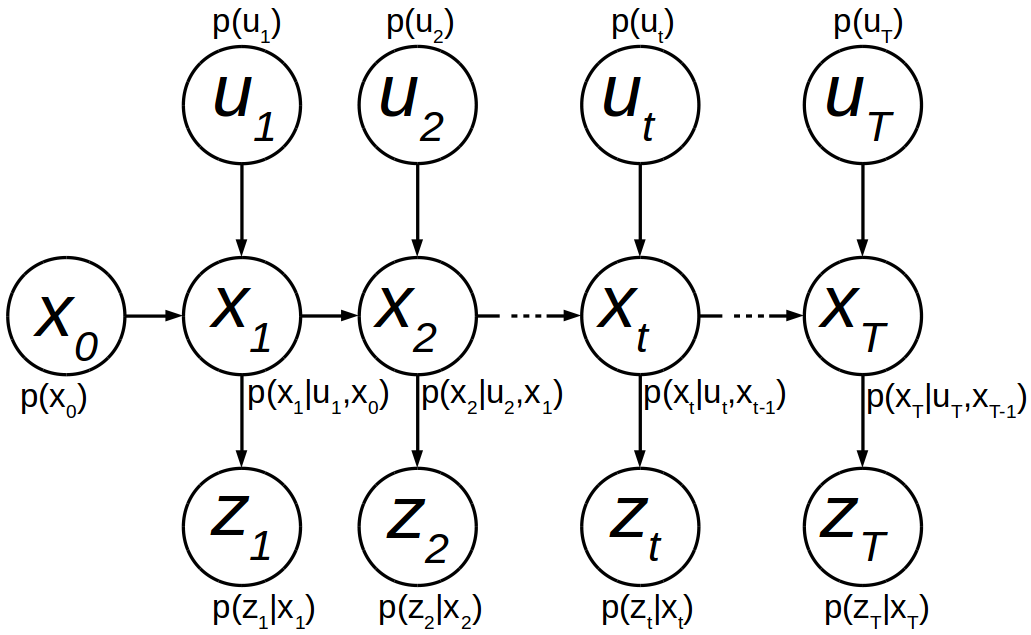
\includegraphics[width=0.7\linewidth]{Figures/bayesnetloc.png}
  \centering
  \caption{Bayesian network of localisation problem}
  \label{fig:loc_bayes}
\end{figure}
\section{Reasoning with a Cluster Graph}\label{sec:cluster}
The Bayesian network in Figure \ref{fig:loc_bayes} is converted to a cluster graph, as shown in Figure \ref{fig:loc_cluster}. The cluster graph allows one to reason about the RVs of the Bayesian network. There are a numerous ways to group the factors to form clusters. In this cluster graph factors $\phi_{\bm{u}_t}, \phi_{\bm{x}_t}$ and $\phi_{\bm{z}_t}$  at each time step $t$  were grouped together to form a cluster $C_t$. The cluster factor of each cluster $C_t$ can be determined as
\begin{equation}
\psi_t(\bm{x}_t, \bm{x}_{t-1}, \bm{u}_t, \bm{z}_t) = \phi_{\bm{x}_t}(\bm{x}_t,\bm{u}_t,\bm{x}_{t-1})\phi_{\bm{z}_t}(\bm{z}_t,\bm{x}_t)\phi_{\bm{u}_t}(\bm{u}_t).
\end{equation}

\begin{figure}
  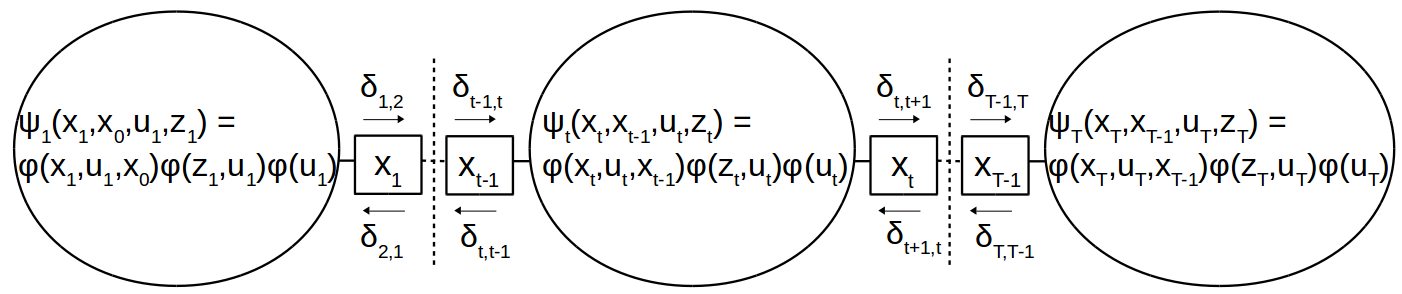
\includegraphics[width=\linewidth]{Figures/loc_clustergraph.png}
  \centering
  \caption{Cluster graph with grouped factors and sepsets}
  \label{fig:loc_cluster}
\end{figure}

Sepsets between clusters are indicated with rectangles and allow clusters to reason about mutual variables by means of message passing. In Figure \ref{fig:loc_cluster} messages associated with sepsets are shown in both directions, but for this causal example only messages in the "forward" direction are calculated. The messages pointing from right to left can also be determined and then used to sent information "backwards" in time which can lead to better estimates of beliefs at previous time steps. The process where messages are sent in both directions are known as smoothing.

The initial belief $bel(\bm{x}_0)$ is known and can be viewed as the only incoming message of cluster $C_1$. One can therefore calculate the messages of the cluster graph in Figure \ref{fig:loc_cluster} by starting at the very left cluster, $C_1$, and then calculate each cluster's outgoing message, in a consecutive order.
Applying Equation \ref{eq:messageOut} to calculate an general outgoing message $\delta_{t,t+1}(\bm{x}_t)$ of a cluster $C_t$, one can observe that
\begin{equation}\label{eq:mesBel}
bel(\bm{x}_t) = \eta\delta_{t,t+1}(\bm{x}_t).
\end{equation}
The observation in Equation \ref{eq:mesBel} and Equation \ref{eq:messageOut} can be used to calculate a belief $bel(\bm{x}_t)$, therefore
\begin{equation}\label{eq:outMes}
\begin{split}
bel(\bm{x}_t) & = \eta \delta_{t,t+1}(\bm{x}_t)\\
& = \eta \int_{\bm{x}_{t-1}}\phi_{\bm{x}_t}(\bm{x}_t,\bm{u}_t,\bm{x}_{t-1})\phi_{\bm{z}_t}(\bm{z}_t,\bm{x}_t)\phi_{\bm{u}_t}(\bm{u}_t)\delta_{t-1,t}(\bm{x}_{t-1})\,d\bm{x}_{t-1}\\
& = \eta \int_{\bm{x}_{t-1}}\phi_{\bm{x}_t}(\bm{x}_t,\bm{u}_t,\bm{x}_{t-1})\phi_{\bm{z}_t}(\bm{z}_t,\bm{x}_t)\phi_{\bm{u}_t}(\bm{u}_t =\bm{U}_t)bel(\bm{x}_{t-1})\,d\bm{x}_{t-1}\\
& = \eta \phi_{\bm{z}_t}(\bm{z}_t,\bm{x}_t)\int_{\bm{x}_{t-1}}\phi_{\bm{x}_t}(\bm{x}_t,\bm{u}_t,\bm{x}_{t-1})bel(\bm{x}_{t-1})\,d\bm{x}_{t-1}.
\end{split}.
\end{equation}
The result of Equation \ref{eq:outMes} can be written in terms of CPDs, therefore
\begin{equation}\label{eq:pgmBayesEq}
bel(\bm{x}_t) = \eta p(\bm{z}_t|\bm{x}_t)\int_{\bm{x}_{t-1}}p(\bm{x}_t|\bm{u}_t,\bm{x}_{t-1})bel(\bm{x}_{t-1})\,d\bm{x}_{t-1}.
\end{equation}
Equation \ref{eq:pgmBayesEq} can be compared to Algorithm \ref{bayesAlg} and it can be seen that the procedure of operations is identical to that of the Bayes filter. This shows that reasoning about the state of a robot in a causal system by means of a PGM will give the same result as when the Bayes filter is used. The method of using the PGM is a very general way to represent the problem and can be considered superior to the Bayes filter, as the PGM can be easily changed by adding or removing nodes. PGMs can also be used to model various systems and is not restricted to the localisation problem.

\chapter{Numerical Integration}\label{sec:numInt}
The previous chapter uses a PGM to reason about the belief $bel(\bm{x}_t)$ in a generic way. This is useful as different methods can easily be implemented to do the operations of Equation \ref{eq:outMes}. In this project the canonical form was used to represent and to do operations on factors. If all the factors of Equation \ref{eq:outMes} can be represented with the canonical form, the result can easily be computed. However, a conditional probability distribution (CPD) that is described by a nonlinear function is usually not a Gaussian distribution and cannot be represented with the canonical form. This section investigates three methods to approximate nonlinear transformations of CPDs as linear transformations which will enable one to approximate the belief in Equation \ref{eq:outMes} as a Gaussian distribution.

\section{Taylor Expansion}
The first method uses Taylor expansion to linearise nonlinear functions associated with CPDs. This is not numerical integration as the functions are linearised and the Jacobian matrix of each function must be determined beforehand.
Equations \ref{eq:linear_taylor} to \ref{eq:Ht} are used to linearise the state transition function $\bm{h}$ and measurement function $\bm{g}$.
The linearised functions can be represented by the canonical form by implementing it in the the result of Equation \ref{eq:linCan}. The state transition function is
\begin{equation}\label{eq:nonLinStateTransFunc}
\bm{x}_t = \bm{g}(\bm{u}_t, \bm{x}_{t-1}) + \bm{\varepsilon}_t,
\end{equation}
where
\begin{equation}
\bm{\varepsilon}_t \sim \mathcal{N}(\bm{\varepsilon}, \bm{0}, R_t).
\end{equation}
The nonlinear function, $\bm{g}$, in Equation \ref{eq:nonLinStateTransFunc} can be linearised by means of Taylor expansion. The state transition in Equation \ref{eq:nonLinStateTransFunc} can now be approximated as
\begin{equation}\label{eq:taylorCanLin1}
\bm{x}_t \approx \bm{g}(\bm{u}_t, \bm{\mu}_{t-1}) + G_t(\bm{x}_{t-1} - 
\bm{\mu}_{t-1}) + \bm{\varepsilon}_t.
\end{equation}
The result of Equation \ref{eq:taylorCanLin1} can be written in the form $\bm{y} = F\bm{x} + \bm{g} + \bm{n}$:
\begin{equation}\label{eq:taylorCanLin2}
\bm{x}_t \approx G_t\bm{x}_{t-1} + (\bm{g}(\bm{u}_t, \bm{\mu}_{t-1}) - G_t\bm{u}_{t-1}) + \bm{\varepsilon}_t.
\end{equation}
By implementing the result of Equation \ref{eq:taylorCanLin2} in Equation \ref{eq:conCanResult}, the state transition distribution $p(\bm{x}_t|\bm{u}_t,\bm{x}_{t-1})$ can be approximated as a Gaussian distribution in canonical form: 
\begin{equation}
\mathcal{C}\left(
\begin{bmatrix}
\bm{x}_t \\
\bm{x}_{t-1} \\
\end{bmatrix};
\begin{bmatrix}
R^{-1}  &  -R^{-1}G_t\\
-G_t^T\Sigma^{-1} & G_t^T R^{-1}G_t
\end{bmatrix}
, 
\begin{bmatrix}
-R^{-1}(\bm{g}(\bm{u}_t, \bm{\mu}_{t-1}) - G_t\bm{u}_{t-1})\\
-G_t^T R^{-1}(\bm{g}(\bm{u}_t, \bm{\mu}_{t-1}) - G_t\bm{u}_{t-1})
\end{bmatrix}
\right).
\end{equation}
The the same procedure can be followed to approximate a measurement CPD, described by a nonlinear function, as a Gaussian distribution. The nonlinear function that describes the measurement CPD is defined as
\begin{equation}\label{eq:nonLinMesFunc}
\bm{z}_t = \bm{h}(\bm{x}_t) + \bm{\zeta}_t,
\end{equation}
where
\begin{equation}
\bm{\zeta} \sim \mathcal{N}(\bm{\zeta}; \bm{0}, Q_t).
\end{equation}
The nonlinear function $\bm{h}$ in Equation \ref{eq:nonLinMesFunc} can be linearised using Taylor expansion. Equation \ref{eq:nonLinMesFunc} can therefore be approximated as
\begin{equation}\label{eq:mesLin1}
\bm{z}_t = \bm{h}(\bm{\overline{\mu}}_t) + H_t(\bm{x}_{t} - 
\bm{\overline{\mu}}_{t}) + \bm{\zeta}_t.
\end{equation}
Equation \ref{eq:mesLin1} is written in the form of $\bm{y} = F\bm{x} + \bm{g} + \bm{n}$, therefore
\begin{equation}\label{eq:mesLin2}
\bm{z}_t = H_t\bm{x}_{t} + (\bm{h}(\bm{\overline{\mu}}_t) - H_t\bm{\overline{\mu}}_{t}) + \bm{\zeta}_t.
\end{equation}
The measurement CPD can be be approximated as a Gaussian distribution by implementing the the result of Equation \ref{eq:taylorCanLin2} in Equation \ref{eq:conCanResult}, therefore:
\begin{equation}
\mathcal{C}\left(
\begin{bmatrix}
\bm{z}_t \\
\bm{x}_{t} \\
\end{bmatrix};
\begin{bmatrix}
Q_t^{-1}  &  -Q_t^{-1}H_t\\
-H_t^T\Sigma^{-1} & H_t^T Q_t^{-1}H_t
\end{bmatrix}
, 
\begin{bmatrix}
-Q_t^{-1}(\bm{h}(\bm{\overline{\mu}}_t) - H_t\bm{\overline{\mu}}_{t})\\
-H_t^T Q_t^{-1}(\bm{h}(\bm{\overline{\mu}}_t) - H_t\bm{\overline{\mu}}_{t})
\end{bmatrix}
\right).
\end{equation}
It is now possible to describe all the factors of Equation \ref{eq:outMes} with the canonical form and therefore one can approximate the belief $bel(\bm{x}_t)$ with the PGM as a Gaussian distribution. This method will give exactly the same result as the EKF. This is due to the fact that both methods use Taylor expansion to linearise the nonlinear functions, $\bm{g}$ and $\bm{h}$. Further, as mentioned before, the procedure of doing operations in the PGM is identical to that of the Bayes filter.

The first technique to approximate a belief as Gaussian distribution is successfully implemented in the PGM. This shows that the generic property of the PGM makes it easy to implement different techniques to do operations.

\section{Unscented Transform}
The unscented transform is used to approximate the result of a Gaussian random variable (RV) passed through a nonlinear function as Gaussian RV. The unscented transform was described in Section \ref{sec:UKF} and is used in the algorithm of the unscented Kalman filter (UKF). The unscented transform can also be viewed as approximating a nonlinear transformation as a linear transformation.

The unscented transform sends carefully chosen Sigma points $\mathcal{X}$ from a Gaussian distribution which is associated with a RV $\bm{x}$, through a nonlinear transformation to produce new Sigma points $\mathcal{Y}$ which is associated with a RV $\bm{y}$. The transformed Sigma points $\mathcal{Y}$ along with weights, $w_c$ and $w_m$ , can be used to estimate the resultant Gaussian distribution of the RV $\bm{y}$. The process of choosing Sigma points and calculating weights were discussed in Section \ref{sec:UKF}.

The mean, $\bm{\mu_{y}}$, covariance, $\Sigma_{\bm{yy}}$, and cross covariance, $\Sigma_{\bm{xy}}$, of the resultant Gaussian distribution can be determined as follows
\begin{equation}\label{eq:mean_y}
\bm{\mu}_{\bm{y}} = \sum_{i = 0}^{2n}w_m^{[i]}\mathcal{Y}^{[i]},
\end{equation}
\begin{equation}\label{eq:Sigma_yy}
\Sigma_{\bm{yy}} = \sum_{i=0}^{2n}w_c^{[i]}\left(\mathcal{Y}^{[i]} - \bm{\mu_{x}}\right) \left(\mathcal{Y}^{[i]} - \bm{\mu_{x}}\right)^T
\end{equation}
and
\begin{equation}\label{eq:Sigma_xy}
\Sigma_{\bm{xy}}= \sum_{i=0}^{2n}w_c^{[i]}\left(\mathcal{Y}^{[i]} - \bm{\mu_{x}}\right) \left(\mathcal{Y}^{[i]} - \bm{\mu_{y}}\right)^T.
\end{equation}
We will now investigate how the results of Equation \ref{eq:mean_y} to Equation \ref{eq:Sigma_xy} can be used to find the linear transformation 
\begin{equation}\label{eq:linearTransform}
\bm{y} \approx F\bm{x} + \bm{g} + \bm{n},
\end{equation}
which is associated with the unscented transform,
where
\begin{equation}
\bm{n} \sim \mathcal{N}(\bm{n}; \bm{0}, \Sigma_{\bm{n}}).
\end{equation}
The mean $\bm{\mu_y}$ of RV $\bm{y}$ can be found by calculating the expected value of Equation \ref{eq:linearTransform}, therefore
\begin{equation}\label{eq:mean_y2}
\begin{split}
\bm{\mu}_y & = \mathcal{E}[F\bm{x} + \bm{g} + \bm{n}]\\
& = F\bm{\mu_x} + \bm{g},
\end{split}
\end{equation}
the covariance matrix $\Sigma_{\bm{yy}}$ associated with RV $\bm{y}$ can be determined by using the definition of covariance defined in Equation \ref{eq:defCovariance}, therefore
\begin{equation}
\begin{split}
\Sigma_{\bm{yy}} & = \mathcal{E}\left[(\bm{y} - \bm{\mu_y})(\bm{y} - \bm{\mu_y})^T\right]\\
& = \mathcal{E}\left[(F\bm{x} + \bm{g} + \bm{n} - F\bm{\mu_x} - \bm{g})((F\bm{x} + \bm{g} + \bm{n} - F\bm{\mu_x} - \bm{g})^T\right]\\
& = F\mathcal{E}\left[(\bm{x} - \bm{u_x})(\bm{x} - \bm{\mu_x}^T)\right]F^T + F\mathcal{E}\left[(\bm{x} - \bm{\mu_x})n^T\right] + \mathcal{E}\left[n(\bm{x} - \bm{\mu_x})^T\right]F^T + \mathcal{E}\left[\bm{nn}^T\right]\\
& = F \Sigma_{\bm{xx}} F^T + \Sigma_{\bm{n}}
\end{split}
\end{equation}
and the cross-covariance $\Sigma_{\bm{xy}}$ can be calculated as
\begin{equation}\label{eq:crossCovariance}
\begin{split}
\Sigma_{\bm{xy}} & = \mathcal{E}\left[(\bm{x} - \bm{\mu_x})(\bm{y} - \bm{\mu}_{\bm{y}})^T\right]\\
& = \Sigma_{\bm{xx}}F^T.
\end{split}
\end{equation}
The parameters of the linear function described in Equation \ref{eq:linearTransform} can now be calculated. Equation \ref{eq:crossCovariance} can be used to determine the matrix $F$, therefore,
\begin{equation}
F = \Sigma_{\bm{xy}}^T\Sigma_{\bm{xx}}^{-1},
\end{equation}\label{eq:detF}
the vector $\bm{g}$ can be determined by using Equation \ref{eq:mean_y2}, therefore
\begin{equation}\label{eq:detg}
\begin{split}
\bm{g} & = \bm{\mu_y} - \Sigma_{\bm{xy}}^T \Sigma_{\bm{xx}}^{-1} \bm{\mu_x}\\
& = \bm{\mu_y} - F\bm{\mu_x}
\end{split}
\end{equation}
and the covariance matrix $\Sigma_n$ can be determined as,
\begin{equation}\label{eq:detSigma_n}
\Sigma_n = \Sigma_{\bm{yy}} - \Sigma_{\bm{xy}}^T\Sigma_{\bm{xx}}^{-1}\Sigma_{\bm{xy}}.
\end{equation} 
The above shows how the unscented transform can be used to estimate a nonlinear transformation as a linear transformation. This can be used to estimate the nonlinear transformations of the state transition CPD and measurement PDF as linear transformations. This allows one to approximate these PDFs as Gaussian PDFs and represent it with the Canonical form.
\section{Monte Carlo Integration}
Monte Carlo integration is the last method that is investigated to approximate a nonlinear transformation as a linear transformation. This technique draws $N$ random points $\mathcal{X}^*$ from a Gaussian distribution, associated with RV $\bm{x}$, and passes them through a nonlinear transformation to produce resultant points $\mathcal{Y}^*$ which are associated with a RV $\bm{y}$. The resultant points $\mathcal{Y}^*$ can be used to calculate the parameters of the Gaussian distribution of the RV $\bm{y}$. The mean $\bm{\mu_y}$ can be calculated with
\begin{equation}
\bm{\mu_y} =  \frac{1}{N}\sum_{i=1}^N\mathcal{Y}^{*[i]},
\end{equation}
the covariance $\Sigma_{\bm{yy}}$ can be calculated with
\begin{equation}
\Sigma_{\bm{yy}} = \frac{1}{N}\sum_{i=1}^N (\mathcal{Y}^{*[i]} - \bm{\mu_y})(\mathcal{Y}^{*[i]} - \bm{\mu_y})^T
\end{equation}
and lastly the cross-covariance $\Sigma_{\bm{xy}}$ can be calculated as
\begin{equation}
\Sigma_{\bm{xy}} = \frac{1}{N}\sum_{i=1}^N (\mathcal{X}^{*[i]} - \bm{\mu_x})(\mathcal{Y}^{*[i]} - \bm{\mu_y})^T.
\end{equation}
The approximated linear transform ($\bm{y} \approx F\bm{x} + \bm{g} + \bm{n}$) from RV $\bm{x}$ to RV $\bm{y}$ can be obtained in the same manner as in the previous section, therefore one can use Equation \ref{eq:detF} to Equation \ref{eq:detSigma_n} again.

\chapter{Results}
All three techniques covered in the previous chapter were successfully implemented in the PGM to approximate the belief of the pose of a robot. This chapter investigates how these techniques compare in terms of accuracy and efficiency. A part of this chapter is based on the work of Duchi~\cite{duchi}.

In order to compare the techniques, a common localisation problem has to be solved using each method. The velocity motion model is used to simulate a moving robot in Python. A Measurement of the robot's pose at each time step is generated with the linear measurement model. Each technique, together with a PGM, is then implemented in Python to solve the same localisation problem and the performance of the techniques are then compared.

\section{Accuracy}
The beliefs, which are determined by implementing the different approximation techniques in the PGM, are now measured in terms of accuracy. First we need to obtain the \textit{ground truth}, which is the desired belief that is wished to be calculated. This desired belief is defined as the optimal Gaussian distribution which describes the uncertainty of a state of a robot. It is not possible to determine a finite answer for the ground truth of this nonlinear system, but a very accurate approximation can be made by using the Monte Carlo technique with a very high sample count.

The next step is to compare the different estimated beliefs with the ground truth. Kullback-Leibler (KL) divergence was method of choice to measure the difference between the Gaussian distributions. Using KL divergence gives a measure of how well one distribution approximates another, where an answer of zero suggests that the distributions are identical. KL divergence is generally defined as
\begin{equation}\label{eq:defKL}
D_{KL}(p_1(\bm{x})||p_2(\bm{x})) = \mathcal{E}\left(\ln\frac{p_1(\bm{x})}{p_2(\bm{x})}\right),
\end{equation}
where the result is a measure of how well $p_2(\bm{x})$ approximates $p_1(\bm{x})$.
The KL divergence can be applied to specifically compare multivariate Gaussian distributions, as this is the nature of all the distributions which is compared. If the distributions $p_1(\bm{x})$ and $p_1(\bm{x})$  in Equation \ref{eq:defKL} are multivariate Gaussian distributions and defined as
\begin{equation}
p_1(\bm{x})  = \mathcal{N}(\bm{x}; \bm{\mu}_1, \Sigma_1),
\end{equation}
and
\begin{equation}
p_2(\bm{x})  = \mathcal{N}(\bm{x}; \bm{\mu}_2, \Sigma_2),
\end{equation}
Then, according to Duchi~\cite{duchi}, Equation \ref{eq:defKL} becomes
\begin{equation}\label{eq:klGauss}
D_{KL}(p_1(\bm{x})||p_2(\bm{x}))= \frac{1}{2}\left(\ln\frac{|\Sigma_2|}{|\Sigma_1|} - n + \text{tr}\left(\Sigma_2^{-1}\Sigma_1\right) + (\bm{\mu}_2 - \bm{\mu}_1)^T \Sigma_2^{-1} (\bm{\mu_2}-\bm{\mu_1})\right),
\end{equation}
where $n$ is the number of dimensions of the multivariate Gaussian distributions.

To compare the accuracy achieved by using the different techniques, it is important that, along with the measurement $\bm{z}_t$ and control vector $\bm{u}_t$, the prior belief $bel(\bm{x}_{t-1})$ which the different estimators receives are identical. One hundred simulations are ran, adhering to the above, and the result of each technique is compared, by using Equation \ref{eq:klGauss}, to the ground truth. The average result can be observed in table \ref{table:kl}, where results that are closer to zero indicate better approximations.

\begin{table}[H]
\center
\begin{tabular}{ |p{6cm}||p{3cm}|}
 \hline
 \multicolumn{2}{|c|}{Kullback-Leibler divergence results} \\
 \hline
 Technique Used & Result\\
 \hline
 1. Monte Carlo (100 samples)   & 0.025\\
 2. Unscented Transform  &  0.169\\
 3. Taylor Expansion &  0.174\\
 4. Monte Carlo (10 samples) & 0.193\\
 \hline
\end{tabular}
\caption{Table to test captions and labels}
\label{table:kl}
\end{table}
Monte Carlo integration draws points randomly where the unscented transform chooses points deterministically. If the concealed distribution is almost a Gaussian distribution, then the unscented transform will be very efficient and accurate. On the other hand if the concealed distribution is highly non-Gaussian then the unscented transform will perform poorly.

\section{Computational Efficiency}
Two methods were used to compare the computational efficiency of these techniques. The first method was to count the number of floating point operations for each technique and compare them in terms of asymptotic complexity. Another comparison was made by measuring the time it takes for each technique to be executed. Combining these results will give a good estimation of how these techniques compare in terms of computational efficiency.

The unscented transform and Taylor expansion are similar in terms of asymptotic complexity.


\chapter{Conclusion}
This project investigates traditional methods to estimate the location of a nonlinear moving robot. First the Kalman filter is applied to find a Gaussian distributed belief of the location of a linear moving robot. The extended and unscented Kalman filters are then applied to estimate the Gaussian belief of a robot with a nonlinear movement, described by the velocity motion model. As the end goal of the project is to compare different techniques of numerical integration, the localisation problem is modelled with a generic probabilistic graphical model (PGM) in the form of a Bayesian network.

Modelling the problem with a PGM has a few advantages, for example it is easy to make changes to the PGM by simply adding or removing nodes, and techniques such as smoothing can also be used. As mentioned before, the PGM is a very generic way to describe the operations as to estimate the location of a causal robotics problem. This allows one to decide how the operations will be performed and in this project the canonical form is used.

It is identified that numerical integration is needed to approximate nonlinear transformations as linear transformations, which allows one to represent nonlinear conditional probability distributions as Gaussian distributions with the canonical form. Two techniques of numerical integration are investigated, namely the unscented transform and Monte Carlo integration.

These techniques are implemented in the PGM that is modelled for the causal localisation problem. The accuracy and efficiency when using the different techniques are then compared. 


\backmatter
\bibliography{mybib}{}

\end{document}\grid
